\documentclass[a4paper]{refart}

\usepackage{makeidx}
\usepackage{ifthen}
\usepackage[T1]{fontenc}

\usepackage[latin1]{inputenc}
\usepackage[english]{babel}
\usepackage{color, xcolor, colortbl}

\usepackage{graphics}
\usepackage[pdftex]{graphicx}
\usepackage[T1,hyphens]{url}
\usepackage{hyperref}

% uncomment this to show Draft
%\usepackage{background}
\usepackage{amsmath}
\usepackage{amssymb,amsfonts,textcomp}
\usepackage{array}
\usepackage{supertabular}
\usepackage{hhline}
\usepackage{chngpage}
\usepackage{float}
\usepackage{listings} 

\lstset{
    breaklines=true,
    stringstyle=\color{blue!40!black},
    belowcaptionskip=1\baselineskip,
    basicstyle=\footnotesize\ttfamily,
    commentstyle=\color{gray},
    keywordstyle=\bfseries\color{purple!40!black},
    frame=none,
    numbers=none,
    xleftmargin=0pt,
    showstringspaces=false,
    numberstyle=\tiny,
    numbersep=5pt,
    tabsize=2,
}
 
\lstdefinestyle{XML}{
    language=xml,
    frame=single,
    numbers=left,
    % emph={food,name,price},emphstyle={\color{magenta}}
    otherkeywords={beginning,property,operator,embedded_function},
}
 
\lstdefinestyle{BASH}{
    language=bash,
    otherkeywords={ls,cd,mkdir}
}

\lstdefinestyle{Cpp}{
    language=C++,
    frame=single,
    numbers=left,
    morecomment=[l][\color{magenta}]{\#},
    otherkeywords={inline, uint64_t, uint32_t, u_char},
}
 
\lstdefinestyle{CONFIG}{
    % language=bash,
    comment=[l]{\#},
    string=[s]{"}{"},
    %otherkeywords={snap-len,license_file_path,Probe-id,thread-nb,logfile,thread-queue,thread-data,input-mode,input-source,file-output,redis-output,kafka-output,socket,data-file,location,retain-files,sampled_report,hostname,port,enabled,domain,socket-descriptor,one-socket-server,enable-proto-without-session-stat,output-channel,enable-IP-fragmentation-report,stats-period,file-output-period,num-of-report-per-msg},
    otherkeywords={ONLINE, OFFLINE, true, false, LAST, FIRST, file, socket},
}

\lstdefinestyle{JSON}{
    string=[s]{"}{"},
    otherkeywords={true, false},
}

\restylefloat{table}
\definecolor{Gray}{gray}{0.9}

\let\textquotedbl="
\def\bs{\char'134 } % backslash in \tt font.
\newcommand{\ie}{i.\,e.}
\newcommand{\eg}{e.\,g.}
\renewcommand\textsubscript[1]{\ensuremath{{}_{\text{#1}}}}
\renewcommand{\arraystretch}{1.5}
\newcommand{\inlineCode}[1]{\texttt{\color{purple!40!black} #1}}
\newcommand{\textQuote}[1]{{\textquotedblleft}#1{\textquotedblright}}
\newcommand{\recommend}{ \marginlabel{$\rightarrow$} }
\newcommand{\note}{ \marginlabel{$\rightarrow$} \underline{Note}: }
\newcommand{\true}{\inlineCode{true} }
\newcommand{\false}{\inlineCode{false} }

%\setcounter{secnumdepth}{4} %take into acount paragraph
\newcommand{\subsubsubsection}[1]{\textbf{#1}}

\hypersetup{
    pdftitle={MMT User Manual},
    pdfsubject={MMT User Manual},
    pdfauthor={Montimage <contact@montimage.com>},
    bookmarksopen=true,
    %color setup    
    colorlinks=false, linkcolor=blue, citecolor=blue, filecolor=blue, urlcolor=blue
}

% Text styles
\newcommand\textstyleAccentuationdiscrte[1]{\textrm{#1}}

\DeclareRobustCommand\cs[1]{\texttt{\char`\\#1}}

\title{MMT User Manual}
\author{\\

\includegraphics[width=1cm,valign=c]{img/icon64x64.png} Montimage \\
~\\
Edgardo Montes de Oca \\
{contact@montimage.com}\\
~\\
MMT-DPI      version 1.7.0\\
MMT-Probe    version 1.4.4\\
MMT-Security version 1.2.11\\
MMT-Operator version 1.7.2}

\date{29/03/2021}
\emergencystretch1em  %

%\pagestyle{myfootings}
%\markboth{MMT User Manual}{MMT User Manual}

\usepackage{fancyhdr}
\usepackage[export]{adjustbox}
\usepackage{graphicx}

\renewcommand{\headrulewidth}{0pt}
\renewcommand{\footrulewidth}{.5pt}
\pagestyle{fancy}
\fancyhf{}
\lfoot{
\includegraphics[width=.75cm,valign=c]{img/icon64x64.png}
       MMT User Manual}
\rfoot{\thepage}

\makeindex 

\setcounter{tocdepth}{2}


\begin{document}

\maketitle

\vfill
\begin{figure}[H]
\hfill

\includegraphics[width=2.5in]{img/mmt_logo.png}
\end{figure}

This user manual presents and explains how to use Montimage monitoring tool (\textbf{MMT}) developed by Montimage's research team.
The manual is suitable for both basic users to use MMT or developers to build their specific applications.

% is an event-based monitoring solution that allows analysing network traffic according to a set of security properties referred to as MMT\_Security properties. The main objective of these properties is to formally specify security goals and/or attack behaviour related to the application or protocol that is being monitored.

For more information please contact us at \url{contact@montimage.com}.

\newpage

\tableofcontents

\newpage


%%%%%%%%%%%%%%%%%%%%%%%%%%%%%%%%%%%%%%%%%%%%%%%%%%%%%%%%%%%%%%%%%%%%%%
\clearpage

\section{Introduction}
\label{Introduction}
\index{Introduction}

Montimage Monitoring Tool (MMT) is a monitoring solution that combines: data capture; filtering and storage; events extraction and statistics collection\footnote{You can try MMT without any installation at \url{http://mmt-cloud.montimage.com}}; and, traffic analysis and reporting. It provides network, application, flow and user level visibility. Through its real-time and historical views, MMT facilitates network security and performance monitoring and operation troubleshooting. MMT-Security engine can correlate network and application events in order to detect operational, security and performance incidents.

% \textbf{MMT\_Security} is a functional and security analysis tool (part of MMT) that verifies application or protocol network traffic traces against a set of MMT\_Security properties. MMT\_Security properties can be either \textit{Security rules} or \textit{Attacks} as described by the following:
% \begin{enumerate}
% \item
% A \textit{Security rule} describes the expected functional or security behaviour of the application or protocol under observation. The non-respect of the MMT\_Security property indicates an abnormal behaviour.
% \item
% An \textit{Attack} describes malicious behaviour whether it is an attack model, a vulnerability or a misbehaviour. Here, the respect of the MMT\_Security property indicates the detection of an abnormal behaviour that might imply the occurrence of an attack.
% \end{enumerate}

This document is divided into 6 sections:

\begin{itemize}
\item
Section~\ref{Introduction} includes this introduction, the tool usage context, a description of the tool{\textquoteright}s global architecture and its main features.

\item Section~\ref{Installing} explains how to install MMT.

\item Section~\ref{configuration} explains how to configure MMT.

\item Section~\ref{Using} explains how to use MMT-Security.

\item Section~\ref{Developers} is dedicated to developers who want to use the libraries for building other applications with specific objectives.

\item Section~\ref{Conclusions} gives a roadmap for future development of the tool.
%\item
%~\nameref{Appendix}: Contains the input files and results of the ARP spoofing example
\end{itemize}

%****************************************************
\subsection{Network and Business Activity Monitoring}

 
\index{scope}\marginlabel{Scope:}
New and more critical vulnerabilities are constantly being introduced by the evolution of the Internet and mobile communications where more and more  critical infrastructures are  becoming open and corporate IT is  being de-materialized (e.g., using cloud services). This is pushing towards the need for more proactive and automated mechanisms for detecting and preventing anomalies due to attacks or misbehaviour.

In this context, Deep Packet Inspection (DPI) is considered as a key element in the shift towards advanced monitoring. DPI is the process of capturing network traffic, analysing and inspecting it in detail to determine accurately what is really happening in the network and applications that communicate. This technology feeds the different monitoring applications with high added value information.

\index{requirements}\marginlabel{Requirements:}Starting from this perception, the requirements of a network/application monitoring system can be summarized as follows:
\begin{enumerate}
\item
\textit{High capturing performance}. It must be able to capture traffic at high speeds and under high traffic volume. This depends on what is to be monitored and where.
\item
\textit{Extensibility}. If new services are integrated in the network, it must be possible to deploy effortlessly new monitoring mechanisms for these specific services. In addition, if new analysis techniques are needed, it should be possible to integrate them as effortlessly as possible.
\item
\textit{Scalability}. It must be able to handle the increase of traffic data that needs to be analysed without performance degradation; due, for instance, to the increase of network link speeds and the number of probes in the network. Scalability can be achieved by reducing the traffic information collected using efficient packet capturing mechanisms, load-balancing and traffic pre-processing.
\item
\textit{Near real time functioning}. It must implement near real time mechanisms in order to quickly detect network security/performance problems and allow timely execution of automated or manual countermeasures.
\item
\textit{Granularity}. It must be able to track the security and performance of each service by capturing and analysing the traffic belonging to the application of interest.
\item
\textit{Diversity}. It must support the network{\textquoteright}s diversity, taking into account different types of network devices from multiple vendors, protocols stacks, and applications providing services to the users.
\item
\textit{Low cost}. It should not use excessive amount of computing, storage, and communication resources so the cost of deploying and operating the monitoring infrastructure remains low for service providers.
\item
\textit{Secure}. It should not add vulnerabilities to the network, or disturb normal network operation.
\end{enumerate}

%****************************************************


%****************************************************
\subsection{MMT Architecture}
 
\index{architecture}\marginlabel{Global architecture:} A high level architecture of the {MMT}{\textquoteright}s frameworks is represented by Figure~\ref{archi}.

\begin{figure}[H]
\centering
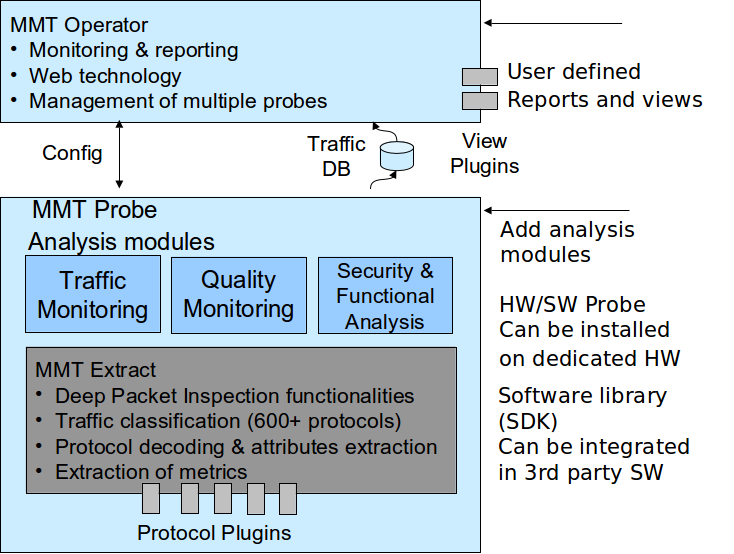
\includegraphics[width=3.8in]{img/archi.png}
\caption{MMT Architecture}\label{archi}
\end{figure}

The integrated {MMT} tool is composed of three complementary, but independent, modules as depicted in this figure.

\textbf{MMT-DPI} is the core packet\footnote{Note that the terms: {\textquotedblleft}packet{\textquotedblright}, {\textquotedblleft}message{\textquotedblright}, {\textquotedblleft}log entry{\textquotedblright} and {\textquotedblleft}event{\textquotedblright} can be considered as equivalent in this document. Here we will use either the term {\textquotedblleft}packet{\textquotedblright} or {\textquotedblleft}event{\textquotedblright} to denote an event in time that is perceived as structured data that can be extracted, classified and analysed.} processing module. It is a C library that analyses network traffic using Deep Packet/Flow Inspection (DPI/DFI) techniques in order to extract hundreds of network and application based events, including: protocols field values, data in messages and logs, network and application QoS parameters and KPIs. MMT-DPI incorporates a plugin architecture for the addition of new protocols and data structures; and, a public API for integrating third party probes (more details given in Section~\ref{Developers}).

\textbf{MMT-Security} is a security analysis engine based on MMT-Security properties described in this document. MMT-Security analyses and correlates network and application events to detect operational and security incidents. For each occurrence of a security property, MMT-Security allows to detect whether it was respected or violated.
The MMT-Security engine has been fully implemented in the context of Montimage{\textquoteright}s research projects. It is the result of previous research work in the network monitoring field and relies on the multi-domain security requirements identified in the context of diverse case studies (more details given in section~\ref{Other}). 

\textbf{MMT-Probe} is a main application that uses MMT-DPI and MMT-Security. It captures packets, makes them available to MMT-DPI and MMT-Security, and receives resulting values (extracted meta data or statistics) to be used for creating reports forwarded to MMT-Operator.

\textbf{MMT-Operator} is a visualization Web application. It allows collecting and aggregating meta data and reports provided by MMT-Probe, and presents them via a graphical user interface (e.g., alarms, line charts). MMT-Operator is customisable: the user is able to define new views or customise the large list of predefined ones. With its generic connector, MMT-Operator can also be integrated with third party traffic probes.



%****************************************************

%****************************************************
\subsection{Features}

\index{architecture}\marginlabel{Main features:} The main features provided by {MMT} are:
\begin{enumerate}
\item
\textit{Granular traffic analysis capabilities}: MMT allows parsing a wide range of protocols and applications and to extract various network and application based traffic performance indicators. The extraction is powered by a plugin architecture for the addition of new protocols and applications.

\item
\textit{Application classification}: Prior to extracting protocol or application attributes, MMT uses DPI techniques for application identification and classification. This is essential when analysing applications that use non-standard port numbers (e.g., P2P, Skype). 

\item
\textit{Rule engine}: MMT-Security introduces a rule engine that allows the detection of complex sequence of events that conventional monitoring does not detect. This is used to monitor: i) access control policies (e.g., that authorized users are authenticated prior to using a critical business application); ii) anomaly or attacks (e.g., excessive login attempts on the application server); iii) performance (e.g., identification of VoIP calls with QoS parameters exceeding acceptable quality thresholds); and, much more.

\item
\textit{Configurable reports}: MMT traffic reports and charts can be configured by the user. The user can edit pre-configured reports and create new ones. Different chart types and graphs can be used including: pie, histograms, time charts, stacked area charts, sequence charts, tables, hierarchical tables, etc.

\item
\textit{Multi-platform solution}: MMT is available and tested on Linux based distributions but portable on Windows. It can be installed as software on commodity hardware or optimized for integration with dedicated probes.

\item
\textit{Modular solution}: MMT is a modular solution composed of four components: MMT-DPI library for the traffic processing and data decoding; MMT-Security engine for property analysis; MMT-Probe application for integrating MMT-DPI and MMT-Security; and MMT-Operator for data aggregation, correlation, reporting, and distributed probe management. It is possible to integrate MMT-DPI and MMT-Security in third party traffic probes and to connect MMT-Operator with existing monitoring systems.
\end{enumerate}
%****************************************************


%%%%%%%%%%%%%%%%%%%%%%%%%%%%%%%%%%%%%%%%%%%%%%%%%%%%%%%%%%%%%%%%%%%%%%

%%%%%%%%%%%%%%%%%%%%%%%%%%%%%%%%%%%%%%%%%%%%%%%%%%%%%%%%%%%%%%%%%%%%%%
\clearpage

\section{Installation}
\label{Installing}

%****************************************************
\subsection{Pre-Requirement}

\subsubsection{Hardware}



%\subsubsubsection{Low Bandwidth}
MMT can run easily on a (personal) computer to process low network traffic, \ie, less than 100 Mbps (mega bit per second). The minimal requirement is that the computer has at least 2 cores of CPU, 2 GB of RAM and 4GB of free hard drive disk. The computer must possess also one NIC (Network Interface Cards) on which MMT captures network traffic. 
Higher network bandwidth requires stronger computer.


To be able to exploit fully capacity of MMT to process very high network bandwidth, one need 
suitable hardware configurations.
MMT can be deployed on a single server or split on separate servers. This section specifies the hardware requirements for the former. For those of the latter, please contact us.

\marginlabel{Network Interface Cards:}
MMT needs at least 2 NICs: one for capturing network traffic and another for administrating. If the probe is to be an active network element (i.e., receives, processes and re-transmits the communication packets) then at least 3 NICs are necessary.

\recommend To achieve the best performance, the capturing NIC should be either Intel X710 or Intel X520 card. These are recommended because they support DPDK that will considerably improve the packet processing. For other hardware architectures, adaptations and tests would need to be performed.


\marginlabel{CPU:} For the best performance, the use of Intel Xeon class server system is recommended, such as Ivy Bridge, Haswell or newer. The larger the CPU cache, the better the performance obtained.

\recommend We recommend having at least 16 cores to process 1 Gbps of traffic. For higher bandwidths other server setups are needed, please contact us for more information.

\marginlabel{RAM:} We recommend using the fastest memory one can buy; and, having one DIMM per channel. One should avoid having 2 or more DIMMs per channel to make sure all memory channels are used to the fullest. It is more expensive to buy 2x16GB than 4x8GB, but with the later, memory access latency increases and the frequency and throughput decreases.

\recommend We recommend having at least 32 GB of RAM to process 1Gps traffic.

\marginlabel{Hard Disk Drive:} If MMT is to write meta data on a hard disk drive, it will do it using a database system (e.g., MongoDB) or files.

\recommend We recommend using a Solid State Drive with at least 20 GB of free space.

\marginlabel{BIOS Settings:}
The following are some recommendations on BIOS settings. Different platforms will have different BIOS naming so the following is mainly for reference:

\begin{enumerate}
    \item  Before starting, consider resetting all BIOS settings to their default.
    \item Disable all power saving options such as: Power performance tuning, CPU P-State, CPU C3 Report and CPU C6 Report.
    \item Select Performance as the CPU Power and Performance policy.
    \item Disable Turbo Boost to ensure the performance scaling increases with the number of cores.
    \item Set memory frequency to the highest available number, NOT auto.
    \item Disable all virtualization options when you test the physical function of the NIC, and turn on \inlineCode{VT-d} if VFIO is required.
\end{enumerate}

\subsubsection{Software}

\marginlabel{Ubuntu LTS 16.04:} This Ubuntu version is recommended to run MMT as MMT has been carefully tested on it. Other Ubuntu version can also run MMT. To run MMT on the other Linux distros and Windows, please contact us.
The example terminal commands used in this manual to prepare MMT running environment is suitable for a machine running Ubuntu LTS 16.04.

\marginlabel{MongoDB >= v3.6} MMT stores meta data using MongoDB. For the use of other database systems please contact us.
To install MongoDB follow steps described in \url{https://docs.mongodb.com/manual/tutorial/install-mongodb-on-ubuntu/}. 
To resume, for Ubuntu 16.04 LTS, one needs to do the following:

\begin{enumerate}
    \item Import the public key used by the package management system:
    
\begin{lstlisting}[style=BASH]
sudo apt-key adv --keyserver hkp://keyserver.ubuntu.com:80 --recv 2930ADAE8CAF5059EE73BB4B58712A2291FA4AD5
\end{lstlisting}

    \item Create a list file for MongoDB and reload the local package database:
    
\begin{lstlisting}[style=BASH]
echo "deb [ arch=amd64,arm64 ] https://repo.mongodb.org/apt/ubuntu xenial/mongodb-org/3.6 multiverse" | sudo tee /etc/apt/sources.list.d/mongodb-org-3.6.list
sudo apt-get update
\end{lstlisting}

    \item Install the MongoDB package:
    
\begin{lstlisting}[style=BASH]
sudo apt-get install -y mongodb-org
\end{lstlisting}

    \item Start MongoDB:
    
\begin{lstlisting}[style=BASH]
sudo service mongod start
\end{lstlisting}
    
    \item Verify that the \texttt{mongod} process has started successfully by checking that the log file \texttt{/var/log/mongodb/mongod.log} contains the line:
    
\begin{lstlisting}[style=BASH]
[initandlisten] waiting for connections on port 27017
\end{lstlisting}
    
    
\end{enumerate}

\marginlabel{NodeJS >= v8.9.1}
The MMT-Operator runs using NodeJS.
To install NodeJS, follow the steps described in \url{https://nodejs.org/en/download/package-manager/}.
To resume, for Ubuntu 16.04 LTS, one needs to do the following:

\begin{enumerate}
    \item Create a list file for NodeJS and reload the local package database:
    
\begin{lstlisting}[style=BASH]
curl -sL https://deb.nodesource.com/setup_8.x | sudo -E bash -
\end{lstlisting}
    
    \item Install NodeJS:
    
\begin{lstlisting}[style=BASH]
sudo apt-get install -y nodejs
\end{lstlisting}
    
    \item Verify that NodeJS was successfully installed:
    
\begin{lstlisting}[style=BASH]
node -v
\end{lstlisting}
    
\end{enumerate}

\marginlabel{Option:} One might need to install the REDIS and/or KAFKA message bus servers if the MMT-Operator is to receive meta data from the MMT-Probe via this type of publish/subscribe systems.


MMT supports the use of the Data Plane Development Kit (DPDK) for high performance capturing of network traffic, e.g., until 40Gbps. To be able to use MMT with other capturing libraries, \eg, netmap, native socket, etc., please contact us.

Before running MMT with DPDK, we need to set the {\textquotedblleft}huge pages{\textquotedblright} option.
    The commands below will reserve 16 GB for MMT-Probe.
Note that this configuration needs to be done after each reboot. For doing it permanently one needs to modify the arguments of the kernel command line.
    
\begin{lstlisting}[style=BASH]
# Each huge page has 2 MB so we need 8192 pages.
# For a single-node system:
echo 8192 > /sys/kernel/mm/hugepages/hugepages-2048kB/nr_hugepages

# For a NUMA system:
echo 4096 > /sys/devices/system/node/node0/hugepages/hugepages-2048kB/nr_hugepages
echo 4096 > /sys/devices/system/node/node1/hugepages/hugepages-2048kB/nr_hugepages
\end{lstlisting}

For this, follow the steps described in \url{http://dpdk.org/doc/guides/linux_gsg/build_dpdk.html} to install DPDK.
To resume, one needs to do the following:
\begin{enumerate}
        \item Install compiler tools:

\begin{lstlisting}[style=BASH]
sudo apt-get update
sudo apt-get install build-essential gcc make python3
\end{lstlisting}

    \item Download DPDK (
    \url{http://fast.dpdk.org/rel/dpdk-16.11.1.tar.xz}):
    
\begin{lstlisting}[style=BASH]
wget http://fast.dpdk.org/rel/dpdk-16.11.1.tar.xz
\end{lstlisting}
    
    \item Decompress the archive and go to the uncompressed DPDK source directory:
    
\begin{lstlisting}[style=BASH]
tar xJf dpdk-16.11.1.tar.xz
cd dpdk
\end{lstlisting}
    
    \item Install DPDK:
    
\begin{lstlisting}[style=BASH]
make install T=x86_64-native-linuxapp-gcc
\end{lstlisting}
     
    \item Load the DPDK driver:
    
\begin{lstlisting}[style=BASH]
sudo modprobe uio
sudo insmod x86_64-native-linuxapp-gcc/kmod/igb_uio.ko
\end{lstlisting}

    \item Bind DPDK to the capturing NIC:
    
\begin{lstlisting}[style=BASH]
# list the status of all NICs on the server:
sudo python3 tools/dpdk-devbind.py --status
# bind capturing NIC eth1 to the igb_uio driver:
sudo python3 tools/dpdk-devbind.py --bind=igb_uio eth1
\end{lstlisting}

\end{enumerate}    

%****************************************************
\subsection{Installation}

\marginlabel{Installing MMT:}
To install MMT do the following steps:

\begin{enumerate}

\item Install MMT:

\begin{lstlisting}[style=BASH]
# Install MMT by order:
# sudo dpkg -i mmt-dpi-<version>.deb
# sudo dpkg -i mmt-security-<version>.deb
# sudo dpkg -i mmt-probe-<version>.deb
# sudo dpkg -i mmt-operator-<version>.deb
# For example:
sudo dpkg -i mmt-dpi_1.6.7.3_Linux_x86_64.deb
sudo dpkg -i mmt-security_1.1.2_7d30208_Linux_x86_64.deb
sudo dpkg -i mmt-probe_1.2.0_7a73b6b_Linux_x86_64.deb
sudo dpkg -i mmt-operator_1.6.2_aa3d383.deb
# Update library path
sudo ldconfig
\end{lstlisting}

\item Verify that MMT was correctly installed:

\begin{lstlisting}[style=BASH]
ls -R /opt/mmt
#=> there must be 6 folders: dpi, examples, operator, plugins, probe, security
\end{lstlisting}

\item Refer to Section~\ref{configuration} to configure MMT as need. 
The configuration files of MMT-Operator and MMT-Probe are located at \path{/opt/mmt/operator/config.json} and \path{/opt/mmt/probe/mmt-probe.conf} respectively. 

For example to use 2 threads of MMT-Probe to capture traffic, 
one should update in \path{/opt/mmt/probe/mmt-probe.conf} the following parameters:


\begin{lstlisting}[style=CONFIG]
# Enable output results to files
file-output {
    enable = true
    ...
}
# Using 2 threads of MMT-Probe
thread-nb    = 2
# Enable MMT-Security
security {
    enable = true
    ...
}
session-report { 
    enable = true
    ...
}
\end{lstlisting}

\end{enumerate}

\marginlabel{Start MMT:}
Execute the following commands to launch the MMT-Operator and the MMT-Probe.

\begin{lstlisting}[style=BASH]
# Start MMT-Operator
sudo mmt-operator

# Start MMT-Probe to monitor traffic on NIC eth0
# run this command on a new terminal
sudo mmt-probe -i eth0

# they can be executed as system services, e.g.,
# sudo service mmt-operator start
# sudo service mmt-probe start

\end{lstlisting}

\marginlabel{View MMT graphical Statistics:}
Open a Web browser, then goto to address \url{http://IP_of_server}, in which, \inlineCode{IP\_of\_server} is IP of administrator NIC of the server installing MMT-Operator.

Log in to MMT-Operator Web interface on the browser using \inlineCode{admin}/\inlineCode{mmt2nm} as username/password. We recommend changing this default password once logged in.


\marginlabel{Uninstalling MMT:}
Execute the following commands to completely remove MMT:

\begin{lstlisting}[style=BASH]
sudo dpkg -r mmt-operator mmt-probe mmt-security mmt-sdk
# Do the following for completely removing all of MMT's execution logs as well as their reports output:
sudo rm -rf /opt/mmt
\end{lstlisting}




%****************************************************



%%%%%%%%%%%%%%%%%%%%%%%%%%%%%%%%%%%%%%%%%%%%%%%%%%%%%%%%%%%%%%%%%%%%%%

\clearpage

\section{Configuration}
\label{configuration}

\subsection{MMT-Probe}

MMT-Probe requires a configuration file for setting different options. 
It can operate in two modes PCAP and DPDK. 
The PCAP mode uses libpcap library, whereas, the DPDK mode uses dpdk library, for packet capturing.  

The execution log of Probe is stored in \inlineCode{syslog} using id \inlineCode{mmt-probe}. 
The log can be viewed using \inlineCode{journalctl -t mmt-probe}.


\subsubsection{Configuration File}

The different available configuration options are given to Probe via a configuration file. 
By default, Probe will try to load the configuration from \inlineCode{./mmt-probe.conf}, or, \inlineCode{/opt/mmt/probe/mmt-probe.conf}
by order of priority. A configuration file can be given to Probe by using \inlineCode{-c} parameter, for example:

\begin{lstlisting}[style=CONFIG]
mmt-probe -c /home/tata/probe.conf
\end{lstlisting}

\note An attribute in the configuration file can be overrided by \inlineCode{-X} parameter.
Multiple \inlineCode{-X} parameters are accepted. 
For example, the following command will override \inlineCode{probe-id} and \inlineCode{source} attribute of \inlineCode{input} block to the coresponding values given after \inlineCode{=} sign.

\begin{lstlisting}[style=CONFIG]
mmt-probe -c /home/tata/probe.conf -Xprobe-id=10 -Xinput.source=/tmp/a.pcap
\end{lstlisting}

To list the attributes that can be overriden, run:

\begin{lstlisting}[style=CONFIG]
mmt-probe -x
\end{lstlisting}

A comment line inside a configuration starts by \inlineCode{\#} sign.

The options are listed in the following:

\marginlabel{ \inlineCode{probe-id}:}
The \inlineCode{probe-id} indicates the identifier of the MMT-Probe. All output report formats contain this identifier. Its value is an integer of 32 bits.

\marginlabel{\inlineCode{license}: }
The \inlineCode{license} indicates the path to a file where the license information is present.

\marginlabel{\inlineCode{stack-type}: }
The \inlineCode{stack-type} indicates protocol suite being used. For now, 1 to monitor Ethernet-based networks, 800 to monitor IEEE802154-based networks, 624 to analyse Linux-cooked-capture pcap files.

\marginlabel{\inlineCode{enable-proto\\-without-session-report}:}
The option indicates whether Probe performs the statistics of the protocols that do not belong to any IP session, such as, ARP, PPP, etc.

\marginlabel{ \inlineCode{enable-ip\\-fragmentation-report}: } 
The option indicates whether Probe performs the statistics of fragmentation of IP packets.

\marginlabel{ \inlineCode{enable-ip-defragmentation}: }
The option indicates whether Probe defragments IP segments before performing any statistics. 

\marginlabel{ \inlineCode{enable-tcp-reassembly}: }
The option indicates whether Probe reassemble TCP segments before performing any statistics.

\marginlabel{ \inlineCode{stats-period}: }
The option indicates the period of sampling in seconds. That is Probe must perform statistics every x seconds. 

\marginlabel{ \inlineCode{dyamic-config}: }
The option indicates whether Probe can be updated its configuration at runtime. If it is enabled, Probe will open an UNIX socket at the given \inlineCode{descriptor} to receive the new configuration parameters.



\marginlabel{ \inlineCode{thread-nb}: }
The option indicates the number of threads the Probe will use for processing packets. It must be a positive number.
Use $0$ to have only one thread to read then analyze packets. Use $x$ to have one thread to read packets and $x$ threads to analyze the packets. 

\marginlabel{ \inlineCode{thread-queue}: }
The option indicates the maximum number of packets that can be queued between the reading thread and an analyzing thread,
thus, total number of packets will be enqueued are \inlineCode{(thread-nb * thread-queues)}.
It has effect only when \inlineCode{thread-nb > 0}.

In case of \inlineCode{input.mode=ONLINE}, 
If a packet is dispatched for a thread having a full queue, then the packet will be dropped.


\marginlabel{ \inlineCode{input}: }
This block configures the input of MMT-Probe. 

\begin{itemize}
  \item \inlineCode{mode} can be either \inlineCode{ONLINE} or \inlineCode{OFFLINE} to indicate that MMT-Probe will analyze respectively either traffic in realtime from a NIC or the traffic being stocked in a pcap file.
      For DPDK, it accepts online \inlineCode{ONLINE} 
      
  \item \inlineCode{source} indicates the source of traffic to be analyze
  \item \inlineCode{snap-len} indicates maximal size of an IP packet, by default 65355 bytes.
  \item \inlineCode{dpdk-option} reserves only for DPDK mode.
\end{itemize}


The options \inlineCode{mode} and \inlineCode{source} need to be specified according to the requirements.

\begin{itemize}
\item{ \inlineCode{mode = ONLINE} } allows {\em near} real-time analysis of network traffic. 
In PCAP mode, the NIC's network interface name needs to be identified, whereas in DPDK mode, the interface port number needs to be identified using the \inlineCode{source} option.
For example:

\begin{lstlisting}[style=CONFIG]
input{
   mode = ONLINE
   # For PCAP it is interface name
   source = "eth0"
   # For DPDK it is  interface port number
   # source = "0"
}
\end{lstlisting}

\item{ \inlineCode{ mode = OFFLINE }} allows analysis of a PCAP trace file. 
The \inlineCode{source} identifies the name of the trace file. 
The offline analysis is only available for the PCAP mode.
For example:


\begin{lstlisting}[style=CONFIG]
input{
   mode   = OFFLINE
   source = "/home/tata/wow.PCAP"
}
\end{lstlisting}
      
\end{itemize}

\marginlabel{ \inlineCode{output}: }
This block configures general output parameters.
\begin{itemize}
  \item \inlineCode{format} is either \inlineCode{JSON} or \inlineCode{CSV} to indicate format of the reports.
  \item Probe maintains a cache of reports to send them by burst tot output channels, such as, to files, to mongoDB, etc.
  The cache will be flushed when its size is over than \inlineCode{cache-max} or periodically designed by \inlineCode{cache-period}.
  
  \item In case of output to files, \inlineCode{cache-period=5} indicates that a new file will be created each 5 seconds if \inlineCode{file-output.samle-file = true} 
\end{itemize}


\marginlabel{ \inlineCode{file-output}: }
This block indicates outputting reports to files.

\begin{itemize}
  \item \inlineCode{enable}: set to \false to disable, \true to enable
  \item \inlineCode{file-name}: name of output files
  \item \inlineCode{output-dir}: path to the folder where output files are written
  \item \inlineCode{sample-file} is either \true or \false to output to multiple sample files or a single file. 
         If \true then a new sample file is created each $x$ seconds given by \inlineCode{output.cache-period} 
  \item \inlineCode{retain-files} indicates number of the latest sample files to be retained if \inlineCode{sample-file = true}.
        Set to $0$ to retain all files. Not that the value of \inlineCode{retain-files} must be greater than \inlineCode{(thread-nb + 1)}
\end{itemize}

For example: 

\begin{lstlisting}[style=CONFIG]
file-output {
    enable       = true  
    output-file  = "data.csv"      
    output-dir   = "/opt/mmt/probe/result/report/online" 
    sample-file  = true
    retain-files = 80
}
\end{lstlisting}

The names of report files are in format \inlineCode{<timestamp>\_<thread-id>\_<name>},
for example, \path{1552302610.832958_0_data.csv}, in which:
\begin{itemize} 
   \item \inlineCode{timestamp} is the moment, in second.microsecond format, of creating the file
   \item \inlineCode{thread-id} is the id of the analyzing thread that generates the file, starting from $0$ to \inlineCode{thread-nb}. Thread $0$ reports status of MMT-Probe, such as, starting time, license information, CPU and memory usages, etc. Threads from $1$ to \inlineCode{thread-nb} report analysis of packets.
   \item \inlineCode{name} is given by \inlineCode{file-output.output-file}
\end{itemize}

Once Probe finished writing reports to a file, it will create a semaphore that is an empty file having the same name with the report file but ending by \path{.sem},
for example, \path{1552302610.832958_0_data.csv.sem}. 


\marginlabel{\inlineCode{redis-output:}}
This configuration bloc indicates that Probe should use REDIS to publish the output. 
The \inlineCode{hostname} and the \inlineCode{port} indicate the address, that can be also an IP, 
 and the port of the redis-server respectively. The \inlineCode{channel} indicates the name of channel to which the reports will be published.
The redis-server needs to be started beforehand.

For example:


\begin{lstlisting}[style=CONFIG]
redis-output
{
    enabled  = true
    hostname = "localhost"
    port     = 6379
    channel  = "report" 
}

\end{lstlisting}

\marginlabel{\inlineCode{kafka-output:}}
This block indicates that Probe should output reports to a topic of kafka bus. 
The kafka-server needs to be started beforehand. For example:



\begin{lstlisting}[style=CONFIG]
kafka-output
{
    enabled  = true
    hostname = "localhost" 
    port     = 9092
    topic    = "report" 
}
\end{lstlisting}


\marginlabel{\inlineCode{mongo-output:}}
This block indicates that Probe should output reports to a collection of mongo database.
The database server needs to be started beforehand. For example:



\begin{lstlisting}[style=CONFIG]
mongodb-output {
    enable     = true
    hostname   = "localhost"
    port       = 27017
    database   = "mmt-data"
    collection = "reports" # name of collection to store reports

    # limit size (megabytes = 1000*1000 bytes) of the collection
    # - set 0 to unlimit
    # - if size of the collection reaches the limit, the oldest reports will be removed to maintain the limit
    limit-size  = 0
}
\end{lstlisting}

\marginlabel{\inlineCode{socket-output:}}
This block indicates that Probe should output report to either a UNIX or internet sockets or both.
The socket server must be started beforehand.

The value of \inlineCode{socket-output.type} can be either \inlineCode{UNIX} for UNIX domain socket type, or \inlineCode{INTERNET} for internet domain socket type, or \inlineCode{BOTH} for using both of two types above.

For example:


\begin{lstlisting}[style=CONFIG]
socket-output
{
    enable = true
    type = BOTH
    descriptor = "/tmp/mmt-probe-output.sock" # required for UNIX domain.
    port = 5000            # Required for Internet domain.
    hostname = "127.0.0.1" # required for Internet domain.
}
\end{lstlisting}

\marginlabel{\inlineCode{dump-pcap:}}
This block indicates that Probe should dump the analyzed packets to files.
For example:


\begin{lstlisting}[style=CONFIG]
dump-pcap
{
    enable       = true
    output-dir   = "/opt/mmt/probe/pcap/"
    
    # List of protocols, separated by comma, must appear in a packet which will be dumped
    protocols    = {"unknown", "http"} 
    period       = 60    # new pcap file is created every x seconds. 0 means default value 3600 seconds
    retain-files = 50    # retains the last x files,
    snap-len     = 65355
}
\end{lstlisting}


\marginlabel{\inlineCode{security}:}
The security output configuration blocs allow specifying the security reporting.

\begin{itemize}
   \item \inlineCode{thread-nb} indicates the number of security threads for each analyzing thread of Probe.
   
   For example, if we have 16 Probe analyzing threads and \inlineCode{ security.thread-nb = x },
   then \inlineCode{(x*16)} security threads will be used .

   If set to zero this means that the security analysis will be performed in the analyzing threads of the probe .

    
   \item \inlineCode{exclude-rules} indicates the range of rules to be excluded from the verification.
   
   The range of rules is in BNF format:  \inlineCode{exclude-rules = "x,y-z"}, in which \inlineCode{x,y, z} are positive numbers.
   
   
   For example, \inlineCode{exclude-rules = "1,3-5,7,50-100"} will exclude the rules having id $1,3,4,5,7,50, 51, \ldots, 100$.
   
   
   
   \item \inlineCode{rules-mask} indicates  the range of rules should be distributed to a specific security thread.
    
   By default, the rules will be distributed increasingly to each thread. 
   For example, given five security rules having id 1, 5, 6, 7, 8 and two security threads, then,
   the first thread will analyzes rules 1, 5 while the second one analyzes rules 6, 7, 8.
   This can be represented by:
   
   \begin{center}
    \inlineCode{rules-mask = "(1:1,5)(2:6-8)"}
   \end{center}  
  
   Generally, the \inlineCode{rules-mask} uses the following BNF format: 
   \begin{center}
   \inlineCode{rules-mask = (thread-index:rule-range)} 
   \end{center}
   
   in which, \inlineCode{thread-index} is  a positive integer;
       \inlineCode{rule-range} is either a positive integer, or a range of numbers (see \inlineCode{exclude-rules}).
   
   For example,  if we have \inlineCode{thread-nb = 3} and
      \inlineCode{ rules-mask = "(1:1,4-6)(2:3)"},
    then, 
      thread 1 verifies rules 1,4,5,6;  
      thread 2 verifies only rule 3; 
      and 
      thread 3 verifies the rest.
   
   \note if we have \inlineCode{thread-nb = 2} and \inlineCode{ rules-mask = "(1:1)(2:3)"}, 
   then only rules 1 and 3 are verified, the other rules are not.

   
   
   \item \inlineCode{output-channel} indicates the destinations of reports. 
   It can be \inlineCode{redis}, \inlineCode{kafka}, \inlineCode{file}, \inlineCode{mongodb}, or, \inlineCode{socket} 
   to write reports to a redis channel, a kafka topic, files, a mongodb collection, or socket respectively.
   
   We can combination of these channels to output reports to different channels, for example,  \inlineCode{output-channel = \{file, mongodb, socket\}}. 
   
   If nothing is specified, the default value is \inlineCode{file}.
   
   \note The reports can be output a channel if the channel is enabled.
   For example, the security reports will be written to file if and only if we have
    \inlineCode{security.output-channel = {file}} and \inlineCode{file-output.enable = true}.
    
    
    
    \item \inlineCode{report-rule-description} indicates whether include rule's description into the alert reports.
    If set to \false, the descriptions will be an empty string in the reports.
    Excluding descriptions will reduce the size of reports.
   
    \item \inlineCode{ignore-remain-flow} indicates whether ignore the security verification on the rest of an IP flow when an alert has been detected.
   
   
   \item The 3 following parameters are specific for MMT-Security to override its default configuration:
    \begin{itemize}
    \item \inlineCode{input.max-message-size = 60000}: size of a message, in bytes, to encapsulate data sending from MMT-Probe to MMT-Security
    \item \inlineCode{security.max-instances = 100000}: maximum number of instances of a rule
    \item \inlineCode{security.smp.ring-size = 1000}: maximum number of messages that will be stored in a ring buffer
    \end{itemize}
    
    
    \item 
    \inlineCode{ip-encapsulation-index} this option selects which IP layer will be analyzed in case there exist IP encapsulation.
    Its value can be one of the followings:
    
    \begin{itemize}
      \item \inlineCode{FIRST}: first IP in the protocol hierarchy
      \item \inlineCode{LAST}:  last IP in the protocol hierarchy
      \item $i$: $i^{th}$  IP in the protocol hierarchy.
   \end{itemize}    
                                     
   For example, given ETH.IP.UDP.GTP.IP.TCP.VPN.IP.SSL,
   
   \begin{itemize}
     \item  \inlineCode{FIRST}, or 1, indicates IP after ETH and before UDP
     \item  \inlineCode{LAST}, or any number >= 3, indicates IP after VPN
     \item  2 indicates IP after GTP and before TCP
   \end{itemize}
                                         
\end{itemize}

For example,
\begin{lstlisting}[style=CONFIG]
security
{    
    enable = true
    thread-nb      = 1  
    exclude-rules  = "(50-100)"
    rules-mask     = "" 
    output-channel = {file, socket}
    report-rule-description = true
    ignore-remain-flow      = true
    input.max-message-size  = 60000
    security.max-instances  = 100000
    security.smp.ring-size  = 1000
    ip-encapsulation-index  = LAST 
}
\end{lstlisting}



\marginlabel{\inlineCode{session-timeout}: }
The  configuration bloc specifies the session timeout in seconds for different types of applications. 
For example:

\begin{lstlisting}[style=CONFIG]
session-timeout 
{     
    # Default timeout (in seconds) for sessions.
    default-session-timeout = 60  
    short-session-timeout =   15
    # This is reasonable for Web and SSL connections especially when long polling is used.
    long-session-timeout =  6000  
    # Usually applications have a long polling period of about 3~5 minutes. This option is for persistent connections like messaging applications and so on
    live-session-timeout  = 1500  
}
\end{lstlisting}	


\marginlabel{\inlineCode{session-report}:}
The configuration bloc enables or disables the reporting of protocols that belong to an IP session. 
The output reports can be reported to a file, redis, kafka or a combination of these channels as being specified in the  \inlineCode{security.output-channel} field. 
For example:

\begin{lstlisting}[style=CONFIG]
session-report
{ 
    enable = true
    output-channel = {}  
    # enable/disable specific reports for specific protocol applications
    ftp  = true
    http = true
    rtp  = false
    ssl  = true
    gtp  = false #specific reports for LTE eNodeB network
    rtt-base = CAPTOR # Order of timestamp's origin that is used to calculate RTT in QOS reports
        # - SENDER: timestamp being marked in packet by its sender, e.g., tcp option TSVal, TSerc
        # This timestamp is available only on certain monitoring protocol, e.g., TCP
        # - CAPTOR: timestamp being marked in packet at the captured moment by its captor (e.g., tcpdump, wireshark)
        # This timestamp is always available.
        # The value of this rtt setting can be one of the followings:
        # - CAPTOR (by default): use only CAPTOR.
        # - SENDER: use only SENDER. Ignore if it is not available
        # - PREFER_SENDER:  use SENDER if it is available, otherwise CAPTOR
}
\end{lstlisting}

\note Currently if \inlineCode{gtp} is enable then the other specific reports must be disable.

\marginlabel{\inlineCode{micro-flows}:}
The  configuration bloc specifies the criteria to use to determine if an IP flow is considered as a micro flow. 

IF an IP flow has some characters, such as, number of packets or bytes, being less than some limits,
 then it will be considered as a micro flow.

A micro-flow is identified by its protocol ID. 
This means that a micro-flow represents several flows having (1) the same protocol ID, and,
(2) their total number of bytes or packets are less than the given thresholds

A single micro flow statistics will not be reported separately, statistics from several micro flows will be aggregated and reported together. 
Aggregating micro flows statistics reduces the number of reports; however, one will lose fine grained information about each flow. 

The micro-flows are not reported periodically but when one of its total number of packets, or bytes, or flows is greater than or equal some limit
given by \inlineCode{report-packet-count}, \inlineCode{report-byte-count} and \inlineCode{report-flow-count},  respectively.

\note Set value of a limit/threshold to zero to unlimit it

For example:



\begin{lstlisting}[style=CONFIG]
micro-flows
{
    enable = true
    packet-threshold =   2     # packets count threshold to consider a flow as a micro flow:
    byte-threshold   = 100     # data volume threshold to consider a flow as a micro flow:

    # a micro-flow will be reported to its output-channel:
    # - at the end of execution of MMT-Probe
    # - or when one of its stats (packets, bytes, flows) is greater than or equal some limit as specified below.
    report-packet-count  =  1000  
    report-byte-count    = 10000
    report-flow-count    =   500

    output-channel = {}
}
\end{lstlisting}

\marginlabel{\inlineCode{data-output}:}
The configuration block is intended for defining the criteria to be used regarding the reporting of specific meta-data. 
For the time being, it only includes criteria to indicate when to include user agent parsing. 
The \inlineCode{include-user-agent} indicates the threshold in terms of data volume for parsing the user agent in Web traffic. 
This configuration bloc will be extended in the future when new reporting needs arise.

For example:


\begin{lstlisting}[style=CONFIG]
data-output
{
    # Indicates the threshold in terms of data volume for parsing the user agent in Web traffic.
    # The value is in kilo Bytes (kB). If the value is zero, this indicates that the parsing of the user agent should be done.
    # To disable the user agent parsing, set the threshold to a negative value (-1). 
    include-user-agent = 32
}
\end{lstlisting}

\marginlabel{\inlineCode{event-report}:}
The  configuration bloc allows to indicate what protocol attributes should be reported when an given event occurred. 
The  \inlineCode{event} indicates the condition that should be satisfied in order to report the attributes; 
and, the \inlineCode{attributes} indicate the application (protocol) attributes that need to be reported when the event occurs. 
Events and attributes should be in "protocol.attribute" format. 

There can be multiple \inlineCode{event-report} configuration blocs. 
Each  bloc is uniquely identified by its name; 
for instance, \inlineCode{event-report report1}, \inlineCode{event-report report2}. 

The output reports can be reported to a file, redis, kafka or a combination of these channels, as specified in the  \inlineCode{security.output-channel} field.

For example: when Probe sees an IP packet having IP.SRC, it will report ARP.AR\_HLN and IP.SRC.
If a packet does not contain an attribute, e.g., ARP.AR\_HLN, the attribute's value is replaced by an empty value (either 0 or "").

For example:


\begin{lstlisting}[style=CONFIG]
event-report ip-event
{
    enable         = true
    event          = "ip.src"
    attributes     = {"arp.ar_hln", "ip.src", "meta.proto_hierarchy"}
    output-channel = {socket}
}
\end{lstlisting}

\marginlabel{\inlineCode{system-report}:}
The configuration bloc defines the  CPU and memory usage reports to be generated. 
The \inlineCode{period} indicates the time-interval for reporting. 
The output reports can be reported to a file, redis, kafka or a combination of these channels, as specified in the  \inlineCode{security.output-channel} field.

For example:


\begin{lstlisting}[style=CONFIG]
cpu-mem-usage
{   
    enable         = true
    period         = 5 
    output-channel = {}
}
\end{lstlisting}

\marginlabel{\inlineCode{behavior}:}
The configuration bloc indicates that the Probe should produce reports
for MMT-Behaviour. 
For example:

\begin{lstlisting}[style=CONFIG]
behaviour
{
    enable       = true
    output-file  = "data.csv"
    output-dir   = "/opt/mmt/probe/result/behaviour/online/"
    retain-files = 300 
}
\end{lstlisting}


\marginlabel{\inlineCode{reconstruct-data ftp}:}
The output configuration bloc indicates that the Probe should reconstruct FTP files and generate reports.
 
To enable the reconstruction, one needs to enable the options \inlineCode{enable-tcp-reassembly = true} and 
\inlineCode{enable-ip-defragmentation = true }.

To enable the reports, the two following options must be enable: \inlineCode{session-report.enable = true} and \inlineCode{session-report.ftp = true}.

The FTP reconstruction reports will be written to \inlineCode{output-channel}, see \inlineCode{security.output-channel}.
 
The FTP reconstruction is only available for the single threaded operation.

For example:


\begin{lstlisting}[style=CONFIG]
reconstruct-data ftp
{   
    enable         = true 
    output-dir     = "/opt/mmt/probe/reconstruct-data/ftp/"
    output-channel = {}
}
\end{lstlisting}


\marginlabel{\inlineCode{reconstruct-data http}:}
The configuration bloc indicates that the Probe should reconstruct the HTTP data. 
It has same requirements as \inlineCode{construct-data ftp}.

For example:


\begin{lstlisting}[style=CONFIG]
condition_report reconstruct_http
{
    enable         = true
    output-dir     = "/opt/mmt/probe/reconstruct-data/http/"
    output-channel = {}
}
\end{lstlisting}


\marginlabel{\inlineCode{radius-report}:}
The  bloc configures the reports for the RADIUS protocol.
 
The \inlineCode{message-id} indicates the kind of message one needs to report:
set to 0 to report all messages;
set to a number (from 1 to 255) to indicate the code of message to report, e.g., 1: Access-Request, 2: Access-Accept, 45: CoA-NAK, etc.
 
The output reports can be reported to a file, redis, kafka or a combination of these channels, as specified in the  \inlineCode{security.output-channel} field.

\begin{lstlisting}[style=CONFIG]
radius-output
{
    enable         = true
    message-id     = 0 
    output-channel = {}  
}
\end{lstlisting}
   

\subsubsection{Execution Parameters}   

Probe can receive several parameters when starting via command line. For example, run \inlineCode{mmt-probe -h} to obtain its list of parameters: 

\begin{lstlisting}[style=BASH]
mmt-probe [<Option>]
Option:
   -v               : Print version information, then exits.
   -c <config file> : Gives the path to the configuration file (default: ./mmt-probe.conf, /opt/mmt/probe/mmt-probe.conf).
   -t <trace file>  : Gives the trace file for offline analyze.
   -i <interface>   : Gives the interface name for live traffic analysis.
   -X attr=value    : Override configuration attributes.
                       For example "-X file-output.enable=true -Xfile-output.output-dir=/tmp/" will enable output to file and change output directory to /tmp.
                       This parameter can appear several times.
   -x               : Prints list of configuration attributes being able to be used with -X, then exits.
   -h               : Prints this help, then exits.
\end{lstlisting}

\subsection{MMT-Operator}

\subsubsection{Configuration File}

The configuration for the MMT-Operator is defined in the \path{/opt/mmt/operator/config.json} file. 
User can given another configuration file to Operator via its running parameter \inlineCode{--config},
for example: \inlineCode{mmt-operator --config=/home/tata/operator.json}.

The configuration file is structured as the following:


\begin{lstlisting}[style=JSON]
{
	"database_server": {
		"host": "localhost",
		"port": 27017
	},
	"redis_input": {
		"host": "localhost",
		"port": 6379
	},
	"kafka_input": {
		"host": "192.168.0.195",
		"port": 2181,
		"ssl.ca.location": "data/kafka-ca.cert"
	},
	"file_input": {
		"data_folder": ["/opt/mmt/probe/result/report/online/", "/mount/probe2/"],
		"delete_data": true,
		"nb_readers": 1
	},
	"input_mode": "file",
	"probe_analysis_mode": "offline",
	"local_network": [
		{
			"ip": "192.168.0.0",
			"mask": "255.255.0.0"
		},{
			"ip": "172.16.0.0",
			"mask": "255.240.0.0"
		},{
			"ip": "10.0.0.0",
			"mask": "255.0.0.0"
		},{
			"ip": "fe80::",
			"mask": "8"
		},{
			"ip": "127.0.0.1",
			"mask": "255.255.255.255"
		}
	],
	"probe_stats_period": 5,
	"buffer": {
		"max_length_size": 30000,
		"max_interval": 5
	},
	"micro_flow": {
		"packet": 1,
		"byte": 64
	},
	"query_cache": {
	  "enable" : true,
	  "folder" : "/tmp/cache/",
	  "bytes" : 10e6,
	  "files" : 9999
	},
	"auto_reload_report": true,
	"retain_detail_report_period": 3600,
	"limit_database_size" :  999999999999,
	"port_number": 8080,
	"log_folder": "/opt/mmt/operator/log/",
	"log" : ["error", "warn", "info"],
	"is_in_debug_mode": true,
	"modules": ["link","network","dpi","security","enodeb"],
	"modules_config" : {
     "enodeb" : {
        "mysql_server" : {
           "host": "localhost",
           "port": 3306,
           "user": "root",
           "password": "montimage",
           "database": "eNodeB"
        }
     }
   }
}
\end{lstlisting}

The content of \path{config.json} can be divided into the following groups:

\marginlabel{Input:} This group specifies how MMT-Operator can receive meta-data generated by the MMT-Probe. The value of \inlineCode{input\_mode} can be one of the following:

\begin{itemize}
  \item \inlineCode{"file"}: MMT-Operator will read meta-data from a file in the folders \inlineCode{data\_folder}. After reading a file, MMT-Operator can delete the file and its semaphore depending on the value defined by \inlineCode{delete\_data}.
  The reading can be accelerated by using several reader in parallel.
  
  \item \inlineCode{"redis"}: MMT-Operator will receive meta-data from a REDIS sever defined by \inlineCode{redis\_server}
  
  \item \inlineCode{"kafka"}: MMT-Operator will receive meta-data from a KAFKA sever defined by \inlineCode{kafka\_server}
\end{itemize}

\marginlabel{Behaviour:}
This group configures the behaviour of the MMT-Operator:

\begin{itemize}
    \item \inlineCode{port\_number} is a port number used to connect to the MMT-Operator web application.

    \item \inlineCode{local\_network} is an array indicating IP ranges of local networks. Each network is given by an IP and network mask.
    
    \item \inlineCode{buffer} limits the size of buffers of MMT-Operator either by (i) the number of elements, \inlineCode{max\_length\_size}, or by the timestamp, \inlineCode{max\_interval}. With a small buffer, MMT-Operator must flush data more frequently to the database and to the Web browser clients.
    
    \item \inlineCode{micro\_flow} indicates retaining detailed information on small flows. This parameter set defines how the MMT-Operator defines micro-flows: maximum number of packets in a flow and maximum number of bytes of data in a flow.
    
    \item \inlineCode{query\_cache} configures the cache of data getting from mongoDB.  
    \item \inlineCode{probe\_stats\_period} is a number, in seconds, indicating the rate of statistic reports from the MMT-Probe. This number must be the same as the value given by \inlineCode{stats\_period} in the configuration file of MMT-Probe.
    
    \item \inlineCode{probe\_analysis\_mode} represents the executing mode of MMT-Probe. Its value must be the same as the value given by \inlineCode{input-mode} in the configuration file of MMT-Probe, \eg, either \inlineCode{"online"} or \inlineCode{"offline"}.
    
    \item \inlineCode{auto\_reload\_report} indicates whether MMT-Operator Web application should refresh periodically its the graphical charts that are displaying, in GUI, to user. This option needs to be \true if one wants view some graphs in realtime.
\end{itemize}

\marginlabel{Maintain Database:} This group contains some thresholds used for the maintenance of the historical database.

\begin{itemize}
  
    \item \inlineCode{retain\_detail\_report\_period} is an interval, in seconds, indicating how long must the MMT-Operator retains information in the collection called \inlineCode{detail} in the database. This collection contains detailed information on each report generated by the MMT-Probe. For example, in the file \path{config.json} above, MMT-Operator will delete the reports that are older than 1 hour.

    \item \inlineCode{limit\_database\_size} is number o bytes indicating the size limit of database. When database overpasses this limit, the oldest documents of each collection will be deleted until the limitation is hold. 
\end{itemize}

\marginlabel{Execution log:} This group configures the execution logs of the MMT-Operator.

\begin{itemize}
  
    \item \inlineCode{log\_folder} is the folder that will contain the execution logs of the MMT-Operator.
    
    \item \inlineCode{log} indicates kinds of log to be written to file. The full list of log can be
    \inlineCode{["error",  "warn", "log", "info"]}
    
    \item \inlineCode{is\_in\_debug\_mode} determines whether the MMT-Operator is running in debug mode, \ie, producing detailed log information. However, this will slow down the MMT-Operator. Its value can be \inlineCode{true} or \inlineCode{false}.
    
\end{itemize}

\marginlabel{Modules:} This group enables or disables some modules as well as their configurations.

\begin{itemize}
  \item \inlineCode{modules} is a list of modules to be enabled.
  
  The full list of modules can be \inlineCode{["link", "network", "dpi", "application", "security", "behavior", "enodeb", "ndn", "video", "sla", "stat"]}
    
  
  \item \inlineCode{module\_config} is specific configuration of each module. 
\end{itemize}

\subsubsection{Execution Parameters}
An configuration option of MMT-Operator can be overridden by giving through running parameter \inlineCode{-X}.

For example, \inlineCode{-Xdatabase\_server.host=10.0.0.2} will change \inlineCode{host} of
\inlineCode{database\_server} bloc to \inlineCode{10.0.0.2}.

The value of \inlineCode{-X} parameter is in format \inlineCode{attribute=value}, where:

\begin{itemize}
   \item \inlineCode{attribute} is path to the attribute to be changed. Dot sign can be used to access to attributes of a bloc, for example,
   
   \inlineCode{-Xmodules\_config.enodeb.mysql\_server.host="10.0.0.2"}.
   
   \item \inlineCode{value} is a primitive value, such as, boolean, number, or string. It must not be an Object or Array.
\end{itemize}

\subsection{MMT-Security}
We can modify the default thresholds of the MMT-Security module in  the file \path{/opt/mmt/security/mmt-security.conf}. The file must be created if it does not exist.

\marginlabel{Input:} 
\begin{lstlisting}[style=CONFIG]
# Maximum size, in bytes, of a report received from the MMT-Probe:
input.max_message_size 3000
\end{lstlisting}

\marginlabel{Security Engine:}
\begin{lstlisting}[style=CONFIG]
# Maximum number of reports that will be stored in a ring buffer:
security.smp.ring_size 1000
# Maximum number of instances of a rule:
security.max_instances 100000
\end{lstlisting}

\marginlabel{Alert:}
\begin{lstlisting}[style=CONFIG]
# Number of consecutive alerts for one rule without the full description. The first alert of a rule always contains a description of its rule. However, to avoid huge outputs, a certain number of consecutive alerts of that rule can be sent without the full description. For instance if value is 20 then the first alert will contain the full description and the next 20 alerts generated by the same rule will not.
# Set value to 0 to include the description in all alerts.
output.ignore_description 20
\end{lstlisting}
%%%%%%%%%%%%%%%%%%%%%%%%%%%%%%%%%%%%%%%%%%%%%%%%%%%%%%%%%%%%%%%%%%%%%%
\clearpage

\section{MMT Security Properties}
\label{Using}


%****************************************************

\subsection{Description}

The MMT-Security properties are intended for formally specifying the occurrence of events that denotes a security rule to be respected or an attack or vulnerability to be avoided. They rely on LTL (Linear Temporal Logic) and are written in XML format. This has the
advantage of being a simple and straight forward structure for the verification and
processing performed by the tool. A graphical editor for creating and editing
MMT-Security properties is under development. In the context of this document, we use the terms of properties and rules interchangeably.


\index{description}\marginlabel{Description:} An MMT-Security properties XML file can contain as many properties as required. The file needs to begin with a
\inlineCode{{\textless}beginning{\textgreater}} tag and end with
\inlineCode{{\textless}/beginning{\textgreater}}. Each property begins with a
\inlineCode{{\textless}property{\textgreater}} tag and ends with
\inlineCode{{\textless}/property{\textgreater}}. A property is a
{\textquotedblleft}general ordered tree{\textquotedblright} and can be
graphically represented as shown in Figure~\ref{rules}:


\begin{figure}[H]
\centering
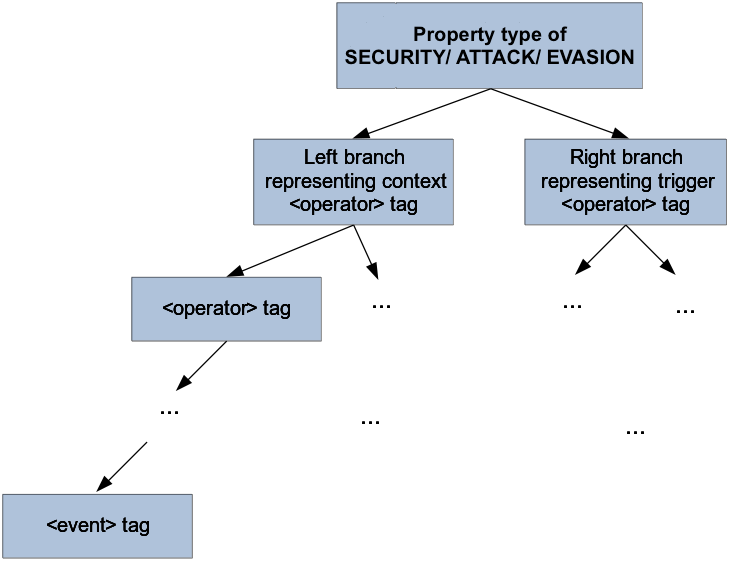
\includegraphics[width=4in]{img/rules.png}
\caption{MMT-Security property structure}\label{rules}
\end{figure}


\index{validation}\marginlabel{Property validation or violation:} The nodes of the property tree are: the property node (required),
operator nodes (optional) and event nodes (required). The property node
is forcibly the root node and the event nodes are forcibly leaf nodes.
In general, the left branch represents the context and the right branch represents
the trigger. This means that the property is found valid when the
trigger is found valid; and the trigger is checked only if the context
is valid. In other words:

\begin{itemize}
\item If the context is verified and the trigger is not, then a property
non-respect instance is detected.

\begin{itemize}
\item In the case of a \inlineCode{SECURITY} rule, this means that the context of the rule has
been found and, since the trigger was not, we conclude that the
\inlineCode{SECUIRTY} rule has been violated.
\item In the case of an \inlineCode{ATTACK} or \inlineCode{EVASION} rule,
this means that the context of an attack has occurred but the trace was
attack free because we did not detect the final trigger.
\end{itemize}
\item If the context and the trigger are verified, then a property
respect instance is detected.

\begin{itemize}
\item In the case of a \inlineCode{SECURITY} rule, this means that the context of the rule has
been found, as well as the trigger. We conclude that the
\inlineCode{SECURITY} rule has been respected.
\item In the case of an \inlineCode{ATTACK} or \inlineCode{EVASION} rule,
this means that the context of an attack has occurred, as well as the
trigger. We conclude that the behavioural attack/evasion has been detected.
\end{itemize}
\end{itemize}

To illustrate how a property is specified, a simplified instance of the Figure \ref{rules}) in XML gives :

\begin{lstlisting}[style = XML, title = General format of a property]
<property value="THEN" delay_units="s" delay_min="0+" delay_max="2" property_id="1" type_property="ATTACK" description="(description of attack)">
    <operator value="THEN" delay_max="1" >
    <event value="COMPUTE" event_id="1"
        description="(description of event 1)"
        boolean_expression="(Boolean expression allowing to detect event 1)"/>
    <event value="COMPUTE" event_id="2"
        description="(description of event 2)"
        boolean_expression="(Boolean expression allowing to detect event 2))"/>
    </operator>
    <event value="COMPUTE" event_id="3"
        description="(description of event 3)"
        boolean_expression="(Boolean expression allowing to detect event 3)"/>
</property>
\end{lstlisting}


\index{note}\note A context can occur before, at the same time or after a
trigger, depending on how the delays or counters attributes are defined (as explained in the next table \ref{prop_att}). To date, we have a library of MMT rules including the following types: 
\begin{itemize}
\item{Uni-packet rules: The events will be verified on the same packet, i.e., the extracted meta-data of one packet satisfy both the context and the trigger conditions.}
\item{Multi-packet, Uni-session rules: The events will be verified in multiple packets but belonging to the same session. This means that the source and destination IP addresses and ports correspond to the same session.}
\item{Multi-session, Uni-probe rules: The events will be verified in multiple packets in multiple sessions based on the reports coming from one single MMT-Probe.}
\item{Multi-session, Multi-probe rules: The events will be verified in multiple packets in multiple sessions based on the reports coming from several MMT-Probes.}
\end{itemize}

\index{propatt}\marginlabel{Property attributes:} The \inlineCode{<property>} tag
contains several attributes, some required, some optional:

\begin{table}[H]
\tablecaption{ Property tag attributes}\label{prop_att}
    \begin{adjustwidth}{-2in}{-.5in}
        \begin{center}
\begin{supertabular}{|m{1.0281599in}|m{1.0281599in}|m{1.0281599in}|m{3.44206in}|}
\hline
\rowcolor{Gray}
 Attribute &
Accepted values &
Req./opt., default value &
Description
\\\hline
property\_id &
Integer &
required &
Property id number, should go from 1 to n where n is the total number of
properties in the XML file. In one or different XML files, two different properties must have two different \inlineCode{property\_id}\\\hline
value &
\inlineCode{"THEN"}%, \inlineCode{"BEFORE"} 
&
required &
A property is a tree and each node can have one or more branches. The
{\textless}property{\textgreater} tag here represents the root of a
tree that can have 2 branches: the context and the trigger.

The value attribute indicates that the left
branch representing the context needs to be valid before, after or at the same time we check the
right branch representing the trigger, depending on the delays defined for the node.
\\\hline
type\_property &
\inlineCode{"ATTACK"},
\inlineCode{"EVASION"},
\inlineCode{"SECURITY"}&
required &
Indicates that the property specifies a potential attack/evasion (or abnormal
behaviour) or that the property specifies a security rule that needs to
be respected.\\\hline
\inlineCode{delay\_min} &
Integer &
optional, default value 0 &
Defines the validity period ([delay\_min, delay\_max]) of the left branch
(e.g. context). 

If we have [a,b] with a=b=0 then the left branch needs to occur in the
same time as the right branch. 

If we have a{\textless}b{\textless}=0 then the right branch needs to
have occurred in the past time interval with respect to the left
branch. 

If we have 0{\textless}=a{\textless}b then the right branch needs to
occur in the future with respect to the left branch. 

If the time runs out before detecting the events concerned then we are
in a TIMEOUT condition, i.e., the context occurs but the trigger never arrived in the specified time interval. This would mean that the property failed.  
Note that in the case that an event should not occur during a certain time interval, we refer to it as TIMEIN instead of TIMEOUT.
The default unit of time used is the second but this can be changed using the attribute delay\_units.
\\\hhline{---~}
delay\_max &
Integer &
optional, default value 0 &
For delay\_min, a + sign before the value (e.g.,  {\textquotedblleft}+0{\textquotedblright}) means strictly greater than the value and for delay\_max a - sign means less than.
\\\hline
delay\_units &
Integer &
optional, default value is {\textquotedblleft}s{\textquotedblright} (seconds) &
Defines the time units used in delay\_min and delay\_max attributes. If default value is not wished then this has to be defined before these two attributes. Possible values are Y,M,D,H,m,s(default),ms or mms.
\\\hline
counter\_max (under development)&
Integer &
optional, default value 0 &
Similar to [delay\_min, delay\_max] we can define [counter\_min,
counter\_max] where the unit is the number of packets analysed. 

If the count runs out before detecting the events concerned, then we are
in, respectively, a COUNTIN or COUNTOUT condition.
\\\hhline{---~}
counter\_min (under development)&
Integer &
optional, default value 0 &
\\\hline
description &
String &
required &
The text that clearly explains what the property is about.\\
\hline
\end{supertabular}
        \end{center}
    \end{adjustwidth}
\end{table}


\begin{table}[H]
\tablecaption{ Property tag attributes (cont.)}\label{prop_attb}
    \begin{adjustwidth}{-2in}{-.5in} 
        \begin{center}
\begin{supertabular}{|m{1.0281599in}|m{1.0281599in}|m{1.0281599in}|m{3.44206in}|}
\hline
\rowcolor{Gray}
 Attribute &
 Accepted values &
 Req./Opt., default value &
 Description
\\\hline
if\_satisfied &
String &
optional &
Defines what action should be performed if the property is satisfied. 
The string gives the name of the function that should be executed (see Reactive Functions~\ref{reactive_functions}).
%\\\hhline{---~}
%if\_not\_satisfied &
%String &
%optional &
\\\hline
%keep\_state &
%One or more event\_id{\textquotedblright}s separated by commas &
%optional &
%Allows indicating what event states should be kept. This is used when a property, for which the context becomes valid, should be able to detect all the triggers that occur in the defined time interval and not be {\textquotedblleft}consumed{\textquotedblright} by the first one.
%\\\hline
\end{supertabular}
        \end{center}
    \end{adjustwidth}
\end{table}



\index{opatt}\marginlabel{Operator attributes:} The {\textless} operator{\textgreater} tag in a property contains
several attributes, some required, some optional:


\begin{table}[H]
\tablecaption{ Operator tag attributes}\label{op_att}
    \begin{adjustwidth}{-2in}{-.5in} 
        \begin{center}
\begin{supertabular}{|m{1.0281599in}|m{1.0281599in}|m{1.0281599in}|m{3.44206in}|}
\hline
\rowcolor{Gray}
 Attribute &
 Accepted values &
 Req./Opt., default value &
 Description
\\\hline
value &
\inlineCode{"THEN"},
\inlineCode{"OR"},
\inlineCode{"AND"},
\inlineCode{"NOT"} &
required &
Operators are used to combine different events and build complex events.
{\textquotedblleft}THEN{\textquotedblright} operator is used to
describe ordered events, {\textquotedblleft}AND{\textquotedblright}
operator is used to describe two events without any order and
{\textquotedblleft}OR{\textquotedblright} operator is used to describe
the occurrence of a least one of the events. {\textquotedblleft}NOT{\textquotedblright} negates the underlying sub-tree.\\\hline
description &
String &
optional &
Gives the text that clearly explains what the complex event is
about.\\\hline
delay\_min &
Integer &
optional, default value 0 &
Same as for the {\textless}property{\textgreater} tag. Note that these
attributes are not to be used for the
{\textquotedblleft}OR{\textquotedblright} and {\textquotedblleft}NOT{\textquotedblright} operators.
\\\hhline{---~}
delay\_max &
Integer &
optional, default value 0 &
\\\hhline{---~}
counter\_max &
Integer &
optional, default value 0 &
\\\hhline{---~}
counter\_min &
Integer &
optional, default value 0 &
\\\hline
repeat\_times (under development) &
Integer &
optional, default value 1 &
Allows detecting the repetition of a complex event occurrence a number of times.\\\hline
\end{supertabular}
        \end{center}
    \end{adjustwidth}
\end{table}

\index{evatt}\marginlabel{Event attributes:} Properties indicate the sequence of events that need to be observed. Events
indicate the conditions that need to be verified on a packet or a set of packets for the event to hold. The {\textless}event{\textgreater} tag in a property
contains several attributes, some required, some optional:


\begin{table}[H]
\tablecaption{Event tag attributes}\label{ev_att}
    \begin{adjustwidth}{-2in}{-.5in} 
        \begin{center}
\begin{supertabular}{|m{1.3941599in}|m{1.0254599in}|m{1.0004599in}|m{3.10736in}|}
\hline
\rowcolor{Gray}
 Attribute &
 Accepted values &
 Req./Opt., default value &
 Description
\\\hline
event\_id &
Integer &
required &
This field allows identifying each event and starts from 1 to n where n is the total number of events in the current property.\\\hline
description &
String &
required &
Gives the text that clearly explains what the event is about.\\\hline
value &
\inlineCode{"COMPUTE"} &
required &
Means that the events need to resolve a Boolean expression that is equal
to \inlineCode{true} or
\inlineCode{false} depending on the
attributes values\\\hline
boolean\_expression &
expression &
required &
A Boolean expression, similar to a Boolean expression in the C language
(explained in the following paragraph).\\\hline
\end{supertabular}
        \end{center}
    \end{adjustwidth}
\end{table}


\index{bool}\marginlabel{Boolean expressions:} The \inlineCode{boolean\_expression} is a logical combination of
{\textquotedblleft}{\textless}protocol
name{\textgreater}.{\textless}field
name{\textgreater}{\textquotedblright} and
{\textquotedblleft}{\textless}number{\textgreater}{\textquotedblright}
with the following operators:
{\textquotedblleft}\&\&{\textquotedblright},
{\textquotedblleft}{\textbar}{\textbar}{\textquotedblright},
{\textquotedblleft}{\textgreater}{\textquotedblright},
{\textquotedblleft}{\textgreater}={\textquotedblright},
{\textquotedblleft}{\textless}{\textquotedblright},
{\textquotedblleft}{\textless}={\textquotedblright},
{\textquotedblleft}=={\textquotedblright},
{\textquotedblleft}!={\textquotedblright},
{\textquotedblleft}+{\textquotedblright},
{\textquotedblleft}-{\textquotedblleft},
{\textquotedblleft}/{\textquotedblright},
{\textquotedblleft}*{\textquotedblright}. Blanks and tabs are ignored.
Note that the {\textquotedblleft}\&\&{\textquotedblright} operator
needs to be written in XML as
{\textquotedblleft}\&amp;\&amp;{\textquotedblright}, 
{\textquotedblleft}{\textless}{\textquotedblright} 
needs to be written as
{\textquotedblleft}\&lt;{\textquotedblright}, etc.


A simple \inlineCode{boolean\_expression} can be of the form: 

\begin{center}
\inlineCode{  (<expression> <operator> <expression>) }
\end{center}

in which, \inlineCode{<expression>} is one of the followings:

\begin{itemize}
    \item \inlineCode{<protocol\_name>.<attribute\_name>}
    \item \inlineCode{<protocol\_name>.<attribute\_name>.<event\_id>}
    \item \inlineCode{<numeric\_value>}
    \item \inlineCode{<string\_value>}
    \item \inlineCode{true}
    \item \inlineCode{false}
    \item embedded function
\end{itemize}


The Boolean expressions must respect some syntax rules:

\begin{itemize}
\item The building bloc needs to start with a
\textQuote{(} and end with a \textQuote{)}. Note that to avoid any ambiguities the quotes should explicitly define how the expression is to be resolved, e.g, A \&\& B {\textbar}{\textbar} C should be written as ((A \&\& B) {\textbar}{\textbar} C) or (A \&\& (B {\textbar}{\textbar} C)).
\item An attribute needs to be identified with its \inlineCode{protocol\_name} and
its \inlineCode{attribute\_name} separated by a dot
\textQuote{.}.
\item If the attribute refers to an attribute value from another event,
then the name needs to be followed by a second
\textQuote{.} and the \inlineCode{event\_id} number of
the event concerned. For instance we can have:

\begin{itemize}
\item \inlineCode{(arp.ar\_op == 0)}
means that the field \inlineCode{arp.ar\_op} should be equal to zero.
\item \inlineCode{(arp.ar\_op == arp.ar\_op.1)} means that the field  
\inlineCode{arp.ar\_op} should be equal to the field \inlineCode{arp.ar\_op} of the event in the same rule with the \inlineCode{event\_id} equal to 1.
\end{itemize}
\end{itemize}


\index{exbool}\marginlabel{Example of a Boolean expression:} For example; the following expression means that the event is valid if
the packet received corresponds to the ARP protocol;
the \inlineCode{ar\_op} is 2; \inlineCode{ar\_sip} is the same as \inlineCode{ar\_tip}
of an event 1; and, \inlineCode{ar\_sha} is different with \inlineCode{ar\_sha} of event 2. Where events 1 and 2 occurred before or will occur after depending on the order that the events should occur (defined by the time intervals specified).

% "((((arp.ar_op == 2)&amp;&amp;(arp.ar_sip == arp.ar_tip.1))&amp;&amp;(arp.ar_sha != arp.ar_sha.2)) &amp;&amp; (ethernet.packet_count != 0))"
\inlineCode{"(((arp.ar\_op == 2)\&amp;\&amp;(arp.ar\_sip == arp.ar\_tip.1)) \&amp;\&amp;(arp.ar\_sha != arp.ar\_sha.2))"}

% \begin{table}[H]
%     \begin{adjustwidth}{-1in}{-.5in} 
% \ \ \ \ \ \ \ \ \ \ \ \ \ \ \ \ \ \ \ \ \ \ \ boolean\_expression={\textquotedbl}(((ARP.OPCODE == 2)\&amp;\&amp;

% \ \ \ \ \ \ \ \ \ \ \ \ \ \ \ \ \ \ \ \ \ \ \ (ARP.SRC\_PROTO == ARP.DST\_PROTO.1))\&amp;\&amp;

% \ \ \ \ \ \ \ \ \ \ \ \ \ \ \ \ \ \ \ \ \ \ \ (ARP.SRC\_HARD == ARP.SRC\_HARD.2)){\textquotedbl}
%     \end{adjustwidth}
% \end{table}

The following table gives a more detailed explanation about the
information that is used in the Boolean expression:


\begin{table}[H]
\tablecaption{ Boolean expressions}\label{bool}
    \begin{adjustwidth}{-2in}{-.5in} 
        \begin{center}
\begin{supertabular}{|m{1.0in}|m{1.0in}|m{4.52616in}|}
\hline
\rowcolor{Gray}
 Name &
 Type &
 Description
\\\hline
protocol\_name &
String &
Indicates the protocol of the packet that we need to inspect.\\\hline
attribute\_name &
String &
Indicates the field of the protocol that we will use for verifying a
condition in the event.\\\hline

numeric\_value &
Integer &
Gives the value that will be used to compare with the packet field
value. Note that the
\inlineCode{protocol\_name} and the
\inlineCode{attribute\_name} allow uniquely
identifying the type of value a field contains (e.g. number, IP
address, MAC address in binary format).

Two specific constants, \inlineCode{true} and \inlineCode{false}, represent respectively a non-zero and zero number.
\\\hline

string\_value & 
String &

Gives a chain of characters, enclosed by ' and ', \eg,
\inlineCode{'GET'}
\\\hline

reference &
Integer &
Indicates that we are to use the data obtained for the field from an
event that occurred before (a previously received packet that validated
the previous event). The name is a number that clearly identifies the
event and needs to be exactly the same as the value given in the
\inlineCode{event\_id} attribute of the corresponding {\textless}event{\textgreater}
tag. Note that one should refer to events that occurred beforehand in the property.\\\hline
\end{supertabular}
        \end{center}
    \end{adjustwidth}
\end{table}

\index{extensions}\marginlabel{Extensions:} Embedded functions can be used to extend the elements used in the Boolean expressions (see section~\ref{Embedded}).

\index{compilation}\marginlabel{Property compilation:} After creating the XML properties, we need to compile them by using the executable \inlineCode{compile\_rule}: 
\begin{lstlisting}[style=BASH]
./compile_rule <rule_name>.so <property>.xml
\end{lstlisting} 
%****************************************************


%****************************************************

\subsection{Embedded Functions}
\label{Embedded}
Embedded functions are functions that allow implementing calculations that are too complicated to define using only classical operators on fields in the Boolean expressions of security properties. One can use existing embedded functions or implement a new function. In both cases, they can be used in the Boolean expressions by using the syntax:

\#<name\_of\_function>(<list of parameters>)

For instance:

\inlineCode{(\#em\_is\_search\_engine( http.user\_agent ) == true)}

where \inlineCode{http} is the protocol name and \inlineCode{user\_agent} is the attribute name (i.e., packet meta-data).

\marginlabel{Implement new\\Embedded Functions:}
The embedded functions must respect the C syntax and are used in Boolean expressions using the syntax described above.
Embedded functions are implemented inside \inlineCode{<embedded\_functions>} tag of the XML rule files and will be compiled together with the rules. 
The input parameters are either of the type \inlineCode{const char * } or \inlineCode{int val}. 
For instance, the \inlineCode{em\_is\_search\_engine} above could be implemented as follows:

\begin{lstlisting}[style=Cpp]
<embedded_functions><![CDATA[
//code C
static inline bool em_is_search_engine(const char *agent){
    if( strstr( agent, "google" ) != NULL )
        return true;
    if( strstr( agent, "bing" ) != NULL )
        return true;
    return false;
}]]></embedded_functions>
\end{lstlisting}

\note: The function name should be prefixed by \inlineCode{em\_} to avoid any confusion with other functions in the system.

One can also implement code into 2 other functions to initialize and free common resource:
\begin{itemize}
    \item \inlineCode{void on\_load()\{ ... \}} is called when the rules inside the XML file being loaded into MMT-Security

    \item \inlineCode{void on\_unload()\{ ... \}} is called when exiting MMT-Security
\end{itemize}


\marginlabel{Pre-implemented\\Embedded Functions:} There exist several embedded functions that have been implemented inside MMT-Security.

\begin{enumerate}
    \item \inlineCode{is\_exist( proto.att )} checks whether an event has an attribute of a protocol, \eg, \inlineCode{is\_exist( http.method )} will return \inlineCode{true} if the current event contains protocol HTTP and attribute \inlineCode{method} has a non-null value, otherwise it will return \inlineCode{false}.

    Normally MMT-Security has a filter that allows an event in a rule to be verified only if any proto.att used in its boolean expression contains value. If one of them has not, the rule will not be verified. This allows to reduce number of verification of boolean expression, thus increases the performance.

    For example, given an event having the following boolean expression:
    
    \begin{center}
    \inlineCode{((ip.src != ip.dst) \&\& (\#em\_check\_URI(http.uri) == 1))}
    \end{center}

    This expression is verified only if \inlineCode{ip.src} and \inlineCode{ip.dst} and \inlineCode{http.uri} are not null, hence only HTTP packets are verified (it does not verify every IP packets).

    However, if one use the following expression, that is totally having the same meaning with the previous one:

    \begin{center}
        \inlineCode{((ip.src != ip.dst) \&\& ((#is\_exist(http.uri) == true ) \&\& (\#em\_check\_URI(http.uri) == 1)))}
    \end{center}
    
    MMT-Security need to verify the expression against any IP packet as the \inlineCode{is\_exist} function tell MMT to exclude \inlineCode{http.uri} from its filter.


    \item \inlineCode{is\_empty( proto.att )}, e.g., \inlineCode{is\_empty(http.uri)} checks whether the string value is empty, i.e., its length is zero.

    \item User can use {\em any standard C functions} as embedded function, \eg, \inlineCode{(\#strstr( http.user\_agent, 'robot') != 0)} to check if \inlineCode{http.user\_agent} contains a sub-string \inlineCode{"robot"}.
    
    
    \note Before using a C function, the library containing that function need to be included.
    The following libraries have been pre-included:

    \begin{lstlisting}[style=Cpp]
#include <string.h>
#include <stdio.h>
#include <stdlib.h>
#include "mmt_lib.h"
#include "pre_embedded_functions.h"
    \end{lstlisting}
    
    Thus when using a function that does not defined inside these libraries, one need to include its library. For example:
\begin{lstlisting}[style=Cpp]
<embedded_functions><![CDATA[
#include <math.h>

static inline bool function em_check( double port ){
    double x = sqrt( port );
    ...
}
]]></embedded_functions>
\end{lstlisting}

\end{enumerate}

\marginlabel{Reactive Functions:}\label{reactive_functions}
Reactive functions allow user perform some action when a rule is satisfied.
The functions will be called each time their rules are satisfied. 
When a security and attack rules are satisfied, they will give \inlineCode{not\_respected} and \inlineCode{detected} verdicts respectively.

To implement and use a reactive function, one need to

\begin{enumerate}
    \item 
implement a C function inside \inlineCode{<embedded\_functions>} tag.
The function has the following format:

\begin{lstlisting}[style=Cpp]
typedef void (*mmt_rule_satisfied_callback)(
  const rule_t *rule,//rule being validated
  int verdict,       //DETECTED, NOT_RESPECTED
  uint64_t timestamp,//moment (by time) the rule is validated
  uint64_t counter,  //moment (by order of message) the rule is validated
  const mmt_array_t * const trace  //messages that validate the rule
);
\end{lstlisting}

\item put the function name in attribute \inlineCode{if\_satisfied} of the rule you want to react. For example: \inlineCode{if\_satisfied="em\_print\_out"}

\begin{lstlisting}[style=Cpp]
<beginning>
<embedded_functions><![CDATA[
static void em_print_out( const rule_info_t *rule, int verdict, uint64_t timestamp, uint64_t counter, const mmt_array_t * const trace ){
   const char* trace_str = mmt_convert_execution_trace_to_json_string( trace, rule );
   printf( "detect rule %d\n%s\n", rule->id, trace_str );
}]]></embedded_functions>

<property value="THEN" delay_units="s" delay_max="0" property_id="10" type_property="EVASION" 
    description="HTTP using a port different from 80 and 8080." if_satisfied="em_print_out">
    <event value="COMPUTE" event_id="1" 
        description="a port different from 80 and 8080"
           boolean_expression="((http.method != '')&amp;&amp;((tcp.dest_port != 80)&amp;&amp;(tcp.dest_port != 8080)))"/>
    <event value="COMPUTE" event_id="2" 
           description="HTTP packet"
           boolean_expression="(ip.src != ip.dst)"/>
</property>
</beginning>
\end{lstlisting}

\end{enumerate}

\marginlabel{High Performance Rules:}
To write a rule having a high performance, one need to:

\begin{itemize}
    \item 
use only the proto.att in boolean expression when need

Please refer to the usage of function \inlineCode{is\_exist} to get an example.

\item Use explicitly the following tcp flags to filter out unwanted verification: tcp.fin, tcp.syn, tcp.rst, tcp.psh, tcp.ack, tcp.urg, tcp.ece, tcp.cwr.

For example, the 2 following boolean expressions have the same meaning:

\inlineCode{(tcp.flags == 4)} and 
\inlineCode{((tcp.flags == 4) && (tcp.rst == 1))}

They both return true when only RST flag of a TCP packet is on, but the latter is better as MMT verifies its rule only when tcp.flags and tcp.rst are not zero. Usually less than about 1\% packets having \inlineCode{tcp.rst != 0}, consequently the rule using the second expression will be verified against only 1\% packets.

\item reduce \inlineCode{delay\_max} of a rule to a suitable value

When having a higher value of \inlineCode{delay\_max} MMT-Security creates more rule instances to correlate different events of different packets. When \inlineCode{delay\_max} is zero, the rule is call simple rule, MMT-Security verifies the rule and gives verdict immediately without creating any rule instances. A simple rule is verified much faster than a complex one that has non-zero \inlineCode{delay\_max}.

\recommend MMT-Security can verify 12400 simple rules or 600 complex rules at 10Gbps.

\item optimize implementation of embedded functions

The embedded functions are called each time their boolean expressions are verified. Consequently, rather than initialize something, for example, connection to database, inside these functions, one can do such a task, only once, inside function \inlineCode{on\_load} then store the connection into a static local variable that will be used inside the embedded functions.

\item always use embedded function with \inlineCode{static inline} keyword

For more information about advantage of inline, please refer to document of gcc: {\em An Inline Function is As Fast As a Macro}.
\end{itemize}
%****************************************************


%****************************************************

\subsection{Example}
\subsubsection{Property without Embedded Functions: ARP Spoofing Example}
\label{arp_example}
In order to provide a complete but easy to understand example, the detection of ARP spoofing is presented here in detail. 

\index{arp}\marginlabel{ARP spoofing:} Address Resolution Protocol (ARP) is a telecommunications protocol used for resolution of network layer addresses into link layer addresses, a critical function in multiple-access networks. ARP was defined by RFC 826 in 1982\footnote{\url{https://en.wikipedia.org/wiki/Address_Resolution_Protocol}}. 
ARP spoofing\footnote{\url{https://en.wikipedia.org/wiki/ARP_spoofing}}(RFC5227\footnote{\url{http://www.networksorcery.com/enp/rfc/rfc5227.txt}}) is a technique used to attack a local-area network (LAN). ARP spoofing may allow an attacker to intercept data frames on a LAN, modify the traffic, or stop the traffic altogether. Figure~\ref{arp} represents an attack by a device using MAC address MAC3 (in red).

\begin{figure}[H]
\centering
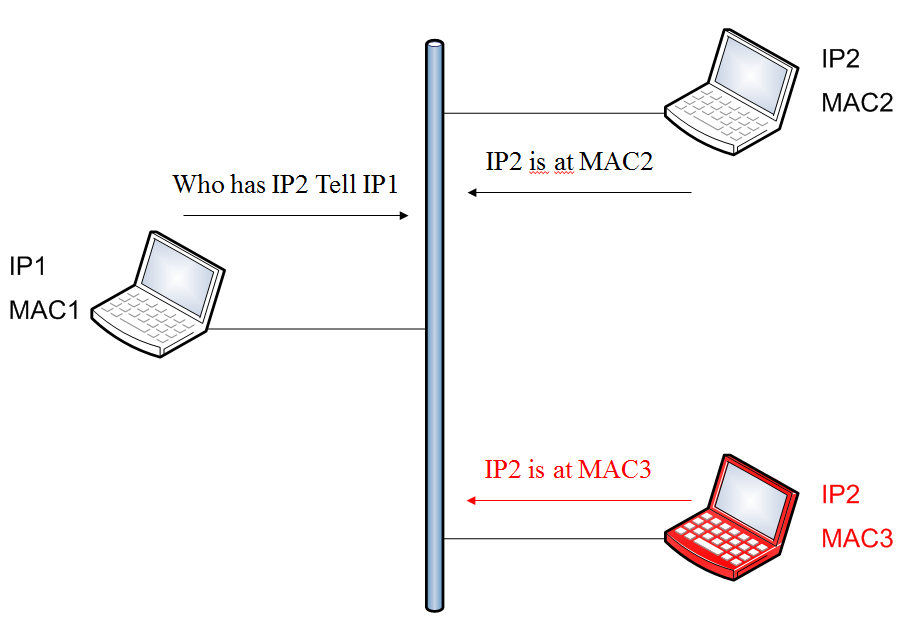
\includegraphics[width=4in]{img/arp_example.png}
\caption{ARP spoofing}\label{arp}
\end{figure}

\index{model}\marginlabel{Attack model:} Following an ARP request (\textit{who has}), a node receives more than one reply with different MAC addresses. This could mean that an IP duplication has been detected that could potentially be an ARP spoofing attack.

This attack behaviour can be specified as follows:

\begin{displaymath} 
 (e\textsubscript{1} ; e\textsubscript{2})\textsubscript{0,4}\hspace{2 mm} AFTER \textsubscript{0,10}\hspace{2 mm} e\textsubscript{3}
\end{displaymath}
Where:


\begin{itemize}
\item \textbf{Event 1} (e\textsubscript{1}): reception of ARP request message
\item \textbf{Event 2} (e\textsubscript{2}): reception of ARP reply message (src MAC2)
\item \textbf{Event 3} (e\textsubscript{3}): reception of ARP reply message with (scr MAC3) != (src MAC2)
\item \textbf{AFTER\textsubscript{0,4}} is an operator indicating that event e\textsubscript{3} occurs after the occurrence of the sequence of events e\textsubscript{1} ; e\textsubscript{2} with a time interval that represents the interval defined in RFC5227 between conflicting ARPs below which a host must not attempt to defend its address. This interval could be reduced or increased to detect spoofing attempts and avoid to many verdicts that are false positives.
\end{itemize}

\bigskip

This security attack is specified by MMT-Security rule as the following:
\lstinputlisting[style=XML]{img/4.arp.xml}

\subsubsection{Property with an Embedded Function: NFS Example}
This property aims to detect the occurrence of the event: "NFS Client uploads a file synchronized to another server" (Fig.~\ref{nfs_upload}). This action can violate the privacy of the data within an organization\rq s network. 
\begin{figure}[H]
\centering
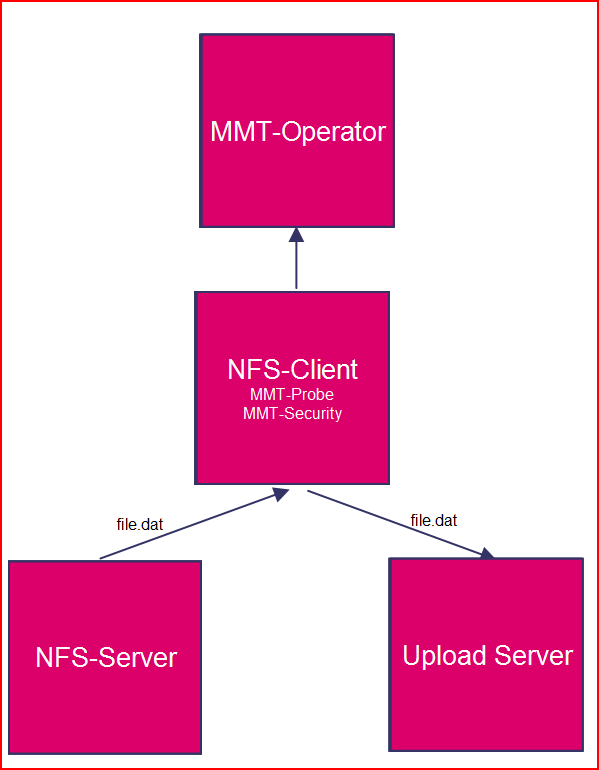
\includegraphics[width=3in]{img/nfs.PNG}
\caption{Upload a file synchronized from NFS Server to another server}
\label{nfs_upload}
\end{figure}

\marginlabel{Using a pre-implemented standard C function:} Suppose that we have one MMT-Probe that assesses NFS traffic as well as HTTP traffic. The attack behaviour can be specified by an MMT rule as follows:
\begin{displaymath} 
(e\textsubscript{1} ; e\textsubscript{2})\textsubscript{0,20}
\end{displaymath}
\lstinputlisting[style=XML]{img/nfs_upload.xml}

Where: 
\begin{itemize}
\item \textbf{Event 1} (e\textsubscript{1}): The reception of an NFS synchronization packet and extraction of the file\rq s name.
\item \textbf{Event 2} (e\textsubscript{2}): The reception of an HTTP packet with the file\rq s name in the payload (verified by the function \inlineCode{\#strstr(tcp.p\_payload, nfs.file\_name.1)}).  
\end{itemize}


\marginlabel{Using a new embedded function:} Suppose that we have two MMT-Probes: One verifies NFS traffic and sends reports to the REDIS bus. The other, analyzes HTTP traffic and uses an Embedded Function to also report to the REDIS bus. The attack behaviour can be specified in an MMT rule as follows:
\begin{displaymath} 
(e\textsubscript{1} ; e\textsubscript{2})\textsubscript{0,0}
\end{displaymath}

\lstinputlisting[style=Cpp]{img/nfs_redis.xml}

Where:
\begin{itemize}
\item \textbf{Event 1} (e\textsubscript{1}): The reception of an HTTP packet with payload length greater than 0.
\item \textbf{Event 2} (e\textsubscript{2}): The embedded function, \inlineCode{em\_check\_nfs\_redis}, is called to:
\begin{itemize}
\item Get the names of all the files synchronized by the NFS Server. These reports are generated by another MMT-Probe and stored in the REDIS bus.   
\item Verify if the name of the file, \textit{file name}, is found in the packet payload. 
\end{itemize}
\end{itemize}



%****************************************************


%****************************************************

\subsection{Other Case Studies}
\label{Other}


Applying MMT-Security to a particular industrial scenario usually involves the following steps: 
\begin{enumerate}
\item
Develop any plugins needed to parse the data to be analysed. Note that parsers for most Internet protocols and applications are already available.
\item
Develop a {\textquotedbl}main.c{\textquotedbl} that will use the libraries to capture and analyse the data.
\item
Define a set of properties that specify the analysis to be performed. 
\end{enumerate}

The tool has been applied or is being applied to several industrial scenarios, such as:
\begin{itemize}
\item Generating broadband reporting for 4G mobile networks (for an equipment manufacturer);
\item Capturing information useful for detecting botnets and other cyber attacks (\url{http://www.acdc-project.eu/} and \url{https://sissden.eu/});
\item Detecting malicious nodes in an ad-hoc network (\url{http://projects.celtic-initiative.org/SAN/});
\item Estimating user Quality of Experience (QoE) of video flows (for an equipment manufacturer);
\item Analysing and fine tuning of delay tolerant networks;
\item Detecting and mitigating attacks in radio protocol communications, Near Field Communication ecosystems and vehicular communications (\url{http://www.itea2-diamonds.org/index.html});
\item Monitoring secure interoperability (\url{http://inter-trust.eu/});
\item Performance analysis for web sites (\url{http://genibeans.com/cgi-bin/twiki/view/Pimi/WebHome/} and \url{http://swept.eu/});
\item Monitoring function for security and performance of Software Defined 5G Mobile Networks, Datacenters, Critical Infrastructures, Cloud infrastructures and services, Cyber-Physical Systems;
\end{itemize}

%ISER, MEVICO/SIGMONA, INQPSIS/NOTTS, PIMI 

%****************************************************

\subsection{Compile MMT-Security Rules}

MMT-Security rules are specified in plain text following an XML format. The rules need to be compiled into a dynamic C library used by MMT.

The compiled rules must put in either \path{./rules} or \paht{/opt/mmt/security/rules}.
The former has higher priority and only one of them will be taken into account by MMT-Security.
Specifically, if MMT-Security found \path{./rules} folder in the current folder executing, it will use the rules inside this folder and
it does not take into account the rules in \path{/opt/mmt/security/rules}.

\marginlabel{Compile rules:}
MMT provides a tool to compile the rules: \path{/opt/mmt/security/bin/compile_rule}. To execute it do:

\begin{lstlisting}[style=BASH]
./compile_rule output_file property_file [-c] [gcc param]
\end{lstlisting}

where:

\begin{enumerate}
\item \inlineCode{output\_file}: is the path of file containing the result that can be either a .c file or .so file.
\item \inlineCode{property\_file}: is the path where the property file can be found.
\item optional parameters: 
    \begin{itemize}
    \item \inlineCode{-c}: will generate only the C code. This option allows manually modifying the generated code before compiling it. 
    After generating the C code, the tool prints out the command that needs to be executed for compiling it.
    
    \item \inlineCode{gcc param}: used to generate the C code, and compile it to obtain the .so file.
                   These parameters will be directly transmitted to the gcc compiler, for example, \inlineCode{"-I/home/tata/include -lmath"}
    \end{itemize}
\end{enumerate}

For example, the following command compiles the rule detecting arp spoofing presented above:

\begin{lstlisting}[style=BASH]
./compile_rule /opt/mmt/security/rules/arp.so arp.xml
\end{lstlisting}

\marginlabel{Obtain information from\\ the compiled rules:} To get some basic information about the compiled rules (such as, ID, description) MMT provides a tool: \path{/opt/mmt/security/bin/rule_info}.

\begin{itemize}
\item By default, the tool will print out the information on all rules located in \path{/opt/mmt/security/rules/}, for instance:

\begin{lstlisting}[style=CONFIG]
/opt/mmt/security/bin/rule_info 
Found 35 rules.
1 - Rule id: 1
	- type            : attack
	- events_count    : 4
	- variables_count : 5
	- variables       : ip.dst (178.13), ip.src (178.12), tcp.dest_port (354.2), tcp.flags (354.6), tcp.src_port (354.1)
	- description     : Several attempts to connect via ssh (brute force attack). Source address is either infected machine or attacker (no spoofing is possible).
	- if_satisfied    : (null)
	- if_not_satisfied: (null)
	- create_instance : 0x7fad94d0be80
	- hash_message    : 0x7fad94d0bd50
	- version         : 1.1.2 (67fa423 - 2017-5-19 18:14:31), dpi version 1.6.8.0 (b3e727b)
2 - Rule id: 10
	- type            : evasion
	- events_count    : 2
	...
...
\end{lstlisting}

\item The tool can also be used to inspect a specific compiled rule by giving the rule path as parameter, for instance:

\begin{lstlisting}
./rule_info /opt/mmt/security/rules/4.arp.so 
Found 1 rule.
1 - Rule id: 4
	- type            : attack
	- events_count    : 3
	- variables_count : 7
	- variables       : arp.ar_op (30.5), arp.ar_sha (30.6), arp.ar_sip (30.7), arp.ar_tip (30.9), ethernet.dst (99.2), ethernet.packet_count (99.4099), ethernet.src (99.3)
	- description     : IPv4 address conflict detection (RFC5227). Possible arp poisoning.
	- if_satisfied    : (null)
	- if_not_satisfied: (null)
	- create_instance : 0x7f5063e7be70
	- hash_message    : 0x7f5063e7bcd0
	- version         : 1.1.2 (67fa423 - 2017-5-19 18:14:34), dpi version 1.6.8.0 (b3e727b)
\end{lstlisting}
\end{itemize}
%%%%%%%%%%%%%%%%%%%%%%%%%%%%%%%%%%%%%%%%%%%%%%%%%%%%%%%%%%%%%%%%%%%%%%

%%%%%%%%%%%%%%%%%%%%%%%%%%%%%%%%%%%%%%%%%%%%%%%%%%%%%%%%%%%%%%%%%%%%%%
\clearpage

\section{MMT-DPI}
\label{Developers}

%****************************************************

\subsection{Extract API}


MMT-DPI is the core packet processing module. It is a C library that analyses network traffic using Deep Packet/Flow Inspection (DPI/DFI) techniques in order to extract hundreds of network and application based events, including: protocols field values, network and application QoS parameters and KPIs. MMT-DPI has a plugin architecture for the addition of new protocols and a public API for integration with third party probes. 

The Figure \ref{extract_lib} shows how a User Program interacts with the library. It captures events that are processed by the library{\textquoteright}s Event Processing Engine. The library will parse the event using the integrated or added Plugins, classify it to determine what type of message it is, extract the needed data from it and send notifications back to the User Program. The classification uses algorithms that allow analysing them and even identify encrypted messages using, for instance, pattern matching and machine learning techniques.


\begin{figure}[H]
\centering
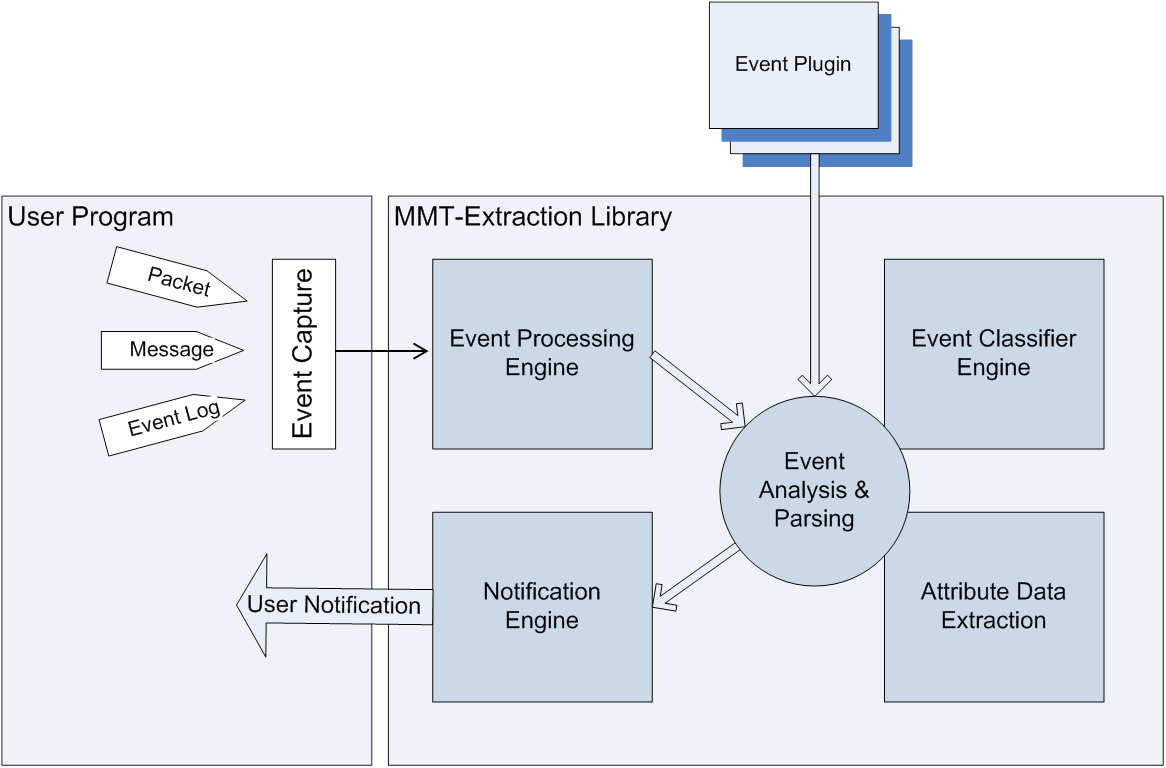
\includegraphics[width=4in]{img/extract_lib.png}
\caption{MMT-DPI Library}\label{extract_lib}
\end{figure}


\subsubsection{Using MMT-DPI in a development project}
In order to use the MMT-DPI library in a development project, one must perform the followings:

\begin{itemize}
\item Include the header file \path{mmt_core.h}: This file is the only one that needs to be included. 
\item By default, the plugins folder locates at \path{/opt/mmt/plugins} after installing MMT-DPI. However you can create a folder called \path{plugins} in the directory where the executable is located, then you should copy the file \path{libmmt_tcpip.so} into \path{plugins} to be able to analyse TCP/IP based network traffic. If one has developped any new MMT-DPI plugin, it must be copied to this \path{plugins} folder. 
Explaining how to add new plugins is described later in this document;
\item Build a \path{main.c} program that uses the library's API (see the following section);
\item Compile the program, linking the MMT-DPI library by using the option: \path{-I/opt/mmt/dpi/include} \path{-L/opt/mmt/dpi/lib} \path{-lmmt_core}
\end{itemize}
\subsubsection{Extraction API description }
The MMT-DPI API is specified in the header files provided with the download package. In the following we will shortly describe the content of the different header files:


\begin{itemize}
\item \path{mmt_core.h}: this is where the core extraction API functions are defined; 
\item \path{data_defs.h}: this is where the data related API functions are defined. In addition, the different data structures that might be used in an integration project are defined here;
\item \path{types_defs.h}: this is where the new data types are defined;
\item \path{extraction_lib.h}: this file contains the generic extraction functions;
\item \path{plugin_defs.h}: this file contains the definitions that can be used for the plugin development.
\end{itemize}

\index{initialization}\marginlabel{Initialization:}
In order to use the MMT-DPI library, one must initialize it by using the following function signature:

\begin{lstlisting}[style=Cpp]
init_extraction () ;
\end{lstlisting}

The initialization returns a positive number on success and zero on failure. It is good practice to always check the return number of \inlineCode{init\_extraction()}.

The following function will create an extraction handler:

\begin{lstlisting}[style=Cpp]
mmt_handler_t *mmt = mmt_init_handler (
        uint32_t stacktype,
        uint32_t options,
        char     *errbuf );
\end{lstlisting}

where the \inlineCode{stacktype} is 1 for 10Mb Ethernet, \inlineCode{options} is 0 and \inlineCode{errbuf} is a \inlineCode{char [1024]} to hold any error message in the case that the return value is \inlineCode{NULL}. The return value is the handle and will be needed by the other functions that need to be called.

For capturing the packets, you can select any library such as: DPDK, PCAP,... In some of our example, we use the PCAP library and, in particular, the following functions (not detailed in this document):
\begin{itemize}
\item    \inlineCode{pcap\_open\_live}
\item    \inlineCode{pcap\_open\_offline}
\item    \inlineCode{pcap\_next}
\item    \inlineCode{pcap\_loop}
\item    \inlineCode{pcap\_close}
\end{itemize}    
    
Each time a packet is recuperated using \inlineCode{pcap\_next} or \inlineCode{pcap\_loop}, it is passed over to the Event Processing Engine using the \inlineCode{packet\_process} function described below in Message processing.

The following function will close the extraction handler and free any previously allocated memory:

\begin{lstlisting}[style=Cpp]
void mmt_close_handler( mmt_handler_t * mmt );
\end{lstlisting}

The following function will close the extraction and free any previously allocated memory:

\begin{lstlisting}[style=Cpp]
int close_extraction ();
\end{lstlisting}

\index{processing}\marginlabel{Message processing:}
MMT-DPI can process network packets in the de-facto PCAP\footnote{PCAP reference} format, raw messages, log messages, etc. 

The following function hands a packet to the core engine of MMT-DPI:

\begin{lstlisting}[style=Cpp]
int packet_process (
    mmt_handler_t *mmt,
    struct pkthdr *header,
    u_char        *packet );
\end{lstlisting}

This function should be called for every packet to process. The \inlineCode{header} parameter of the function is a pointer to the meta-data of the message that include the message arrival time, the message length, etc. The \inlineCode{packet} parameter of the function is a pointer to the message data. The \inlineCode{packet\_process} function will return a positive value on successful processing. Zero is returned if an internal error is encountered, although this should never happen.

\index{registring}\marginlabel{Registering extraction attributes:}
The MMT-DPI library allows registering attributes for extraction. This limits the extraction overhead since only the data that is needed is recuperated. Attributes are fields in a network packet, specific data in a log entry, etc. 


The any of the following two functions can be used to register an attribute for extraction:

\begin{lstlisting}[style=Cpp]
void register_extraction_attribute (
    mmt_handler_t *mmt,
    uint32_t       protocol_id, 
    uint32_t       attribute_id );
\end{lstlisting}

\begin{lstlisting}[style=Cpp]
void register_extraction_attribute_by_name (
    mmt_handler_t *mmt,
    const char    *proto_name,
    const char    *attribute_name);
\end{lstlisting}

An attribute is identified by the protocol and attribute id or names. If the registration succeeds, a positive value will be returned; zero is returned on failure.

The following function allows verifying if an attribute, identified by its protocol and attribute identifiers, is already registered:

\begin{lstlisting}[style=Cpp]
int is_registered_attribute (
        mmt_handler_t *mmt,
        uint32_t       protocol_id,
        uint32_t       attribute_id );
\end{lstlisting}

This function will return a positive value if the attribute is already registered.


The any of the two following functions allow unregistering an attribute:

\begin{lstlisting}[style=Cpp]
int unregister_extraction_attribute (
    mmt_handler_t *mmt,
    uint32_t       protocol_id,
    uint32_t       attribute_id );
\end{lstlisting}

\begin{lstlisting}[style=Cpp]
int unregister_extraction_attribute_by_name (
    mmt_handler_t *mmt,
    uint32_t       proto_name,
    uint32_t       attribute_name );
\end{lstlisting}

If the unregistration succeeds, a positive value will be returned.

To recuperate the data in an attribute, any of the following two functions will return a pointer to the data if it was detected in the current event (i.e., the current packet that is being analysed). If the attribute or data does not exist for the current event then \inlineCode{NULL} will be returned.

\begin{lstlisting}[style=Cpp]
void * get_attribute_extracted_data (
    mmt_handler_t *mmt,
    uint32_t       protocol_id,
    uint32_t       attribute_id);
\end{lstlisting}

\begin{lstlisting}[style=Cpp]
void * get_attribute_extracted_data_by_name (
    mmt_handler_t *mmt,
    const char    *protocol_name,
    const char    *attribute_name );
\end{lstlisting} 

\index{callbacks}\marginlabel{Registering callbacks:}
The MMT-DPI library allows registering callback functions. A registered callback function will be called following the extraction of attributes whenever a packet is processed. 


The following function allows registering a packet handler:

\begin{lstlisting}[style=Cpp]
int register_packet_handler (
    mmt_handler_t                  *mmt,
    int                             handler_id,
    generic_packet_handler_callback function,
    u_char                         *args );
\end{lstlisting}

A packet handler is a callback that will be called each time a packet is processed. If needed, the user can provide a pointer to an argument that will be passed to the callback function when it is called. The callback function is associated with an identifier that should be unique, i.e., two callback functions cannot have the same identifier. This function will return a positive value upon success.

To verify that a packet handler callback function is registered with a given identifier, one can use the following function:

\begin{lstlisting}[style=Cpp]
int is_registered_packet_handler (
        mmt_handler_t  *mmt,
        int             handler_id );
\end{lstlisting}




This function returns a positive value if a registered callback function is found for the provided identifier.




In order to unregister an already registered packet handler one can use:




\begin{lstlisting}[style=Cpp]
int unregister_packet_handler (
        mmt_handler_t *mmt,
        int            handler_id );
\end{lstlisting}




In addition to packet handlers, it is possible to register a callback function to be called when an attribute is detected. This can be done with the following function:




\begin{lstlisting}[style=Cpp]
int register_attribute_handler (
        mmt_handler_t             *mmt,
        uint32_t                   protocol_id,
        uint32_t                   attribute_id,
        attribute_handler_function handler_fct,
        void                      *handler_condition,
        void                      *user_args );
\end{lstlisting}




This function allows registering an attribute handler that is a callback that will be called when the attribute defined by the given protocol and attribute ids is detected (i.e, not NULL). If needed, the user can provide a pointer to an argument that will be passed to the callback function when it is called. In the current version the parameter defined by \inlineCode{handler\_condition} is not implemented and should be set to NULL. This function will return a positive value upon success.


The following function registers an attribute handler given by its protocol and attribute names:


\begin{lstlisting}[style=Cpp]
int register_attribute_handler_by_name (
        mmt_handler_t *mmt,
        const char    *protocol_name,
        const char    *attribute_name,
        attribute_handler_function handler_fct,
        void *handler_condition,
        void *user_args);
\end{lstlisting}

To verify that an attribute handler is registered, one can use the following function:

\begin{lstlisting}[style=Cpp]
int has_registered_attribute_handler (
        mmt_handler_t *mmt,
        uint32_t       protocol_id,
        uint32_t       attribute_id );
\end{lstlisting}

This function returns a positive value if a handler is already registered with the attribute defined by its protocol and attribute identifiers.

In order to unregister an already registered attribute handler one can use:

\begin{lstlisting}[style=Cpp]
int unregister_attribute_handler (
        mmt_handler_t * mmt,
        long protocol_id,
        long attribute_id );
\end{lstlisting}

\begin{lstlisting}[style=Cpp]
int unregister_attribute_handler_by_name (
        mmt_handler_t *mmt,
        const char    *protocol_name,
        const char    *attribute_name );
\end{lstlisting}


\index{functions}\marginlabel{Data functions:}
In addition to the core functions presented so far, MMT-DPI provides a number of utility functions to assist the user of the library. 

The following function returns the protocol name for a given numeric identifier:

\begin{lstlisting}[style=Cpp]
const char * get_protocol_name_by_id (
        mmt_handler_t *mmt,
        uint32_t       protocol_id );
\end{lstlisting}

NULL is returned if the given identifier does not correspond to any configured protocol. 


The following function returns the identifier of the protocol for a given name:

\begin{lstlisting}[style=Cpp]
long get_protocol_id_by_name (
        mmt_handler_t *mmt,
        const char    *protocol_name );
\end{lstlisting}

Zero is returned if the given name does not correspond to any configured protocol. 


The following function indicates if the attribute exists for given protocol and attribute ids.


\begin{lstlisting}[style=Cpp]
int is_protocol_attribute (
        mmt_handler_t *mmt,
        uint32_t       protocol_id,
        uint32_t       attribute_id );
\end{lstlisting}



The following function returns the name of the attribute corresponding to the given protocol and attribute identifiers:

\begin{lstlisting}[style=Cpp]
const char * get_attribute_name_by_protocol_and_attribute_ids (
        mmt_handler_t *mmt,
        uint32_t       protocol_id,
        uint32_t       attribute_id );
\end{lstlisting}

NULL is returned if there is no attribute corresponding to the given identifiers. 


The following function returns the identifier of the attribute corresponding to the given protocol and attribute names:

\begin{lstlisting}[style=Cpp]
long get_attribute_id_by_protocol_and_attribute_names (
        mmt_handler_t *mmt,
        const char    *protocol_name,
        const char    *attribute_name );
\end{lstlisting}

Zero is returned if there is no attribute corresponding to the given names. 


The following function returns the identifier of the attribute corresponding to the given protocol id and attribute name:

\begin{lstlisting}[style=Cpp]
long get_attribute_id_by_protocol_id_and_attribute_name (
        mmt_handler_t *mmt,
        uint32_t       protocol_id,
        const char    *attribute_name );
\end{lstlisting}

Zero is returned if there is no attribute corresponding to the given parameters. 


The following function returns the identifier of the data type of the attribute corresponding to the given protocol and attribute identifiers:

\begin{lstlisting}[style=Cpp]
long get_attribute_data_type (
        mmt_handler_t *mmt,
        uint32_t       protocol_id,
        uint32_t       attribute_id );
\end{lstlisting}

Zero is returned if there is no attribute corresponding to the given parameters. 


The following function returns the data size, in number of bytes, of the attribute corresponding to the given protocol and attribute identifiers:

\begin{lstlisting}[style=Cpp]
int get_data_size_by_proto_and_field_ids (
        mmt_handler_t *mmt, 
        uint32_t       protocol_id, 
        uint32_t       attribute_id );
\end{lstlisting} 

Zero is returned if there is no attribute corresponding to the given parameters. 


The following function returns the data size of the given MMT data type:

\begin{lstlisting}[style=Cpp]
int get_data_size_by_data_type (
        mmt_handler_t *mmt,
        int            data_type );
\end{lstlisting}

Zero is returned if the data type is unknown.


The following function returns the position in the message of the attribute corresponding to the given protocol and attribute identifiers:

\begin{lstlisting}[style=Cpp]
int get_field_position_by_protocol_and_field_ids (
        mmt_handler_t *mmt,
        uint32_t       protocol_id,
        uint32_t       attribute_id );
\end{lstlisting}

For attributes where the position depends on the content of the message, \inlineCode{POSITION\_NOT\_KNOWN} (value -1) will be returned. The position is defined as the byte offset from the beginning of the packet.


%****************************************************

\subsection{Building the main}

To build a main that uses the MMT-DPI and MMT-Security libraries one should carefully study the \path{ARP_probe} example (Sec.~\ref{arp_example}). The main steps that need to be followed for building a \path{main.c} are:

\begin{enumerate}

\item Implement a callback function that will be called each time MMT-DPI parse successfully a packet. In this function, one need to retrieve value of protocol attributes from MMT-DPI and pass them to MMT-Security by calling function \inlineCode{mmt\_sec\_process}.

% \begin{lstlisting}[style=Cpp]
% int packet_handler( const ipacket_t *ipacket, void *args ) {
%     int i;
%     mmt_sec_handler_t *handler = (mmt_sec_handler_t *)args;
%     message_t *msg = create_message_t();	
    
%     msg->timestamp = mmt_sec_encode_timeval( &pkt->p_hdr->ts );
%     msg->counter   = pkt->packet_id;
    
%     //get a list of proto/attributes being used by mmt-security
%     for( i=0; i<proto_atts_count; i++ )
%     	dpi_message_set_data( pkt, proto_atts[i]->dpi_type, msg, proto_atts[i]->proto_id, proto_atts[i]->att_id );
    
%     //if there is no interested information => free the created msg
%     if( msg->elements_count == 0 )
%         free_message_t( msg );
%     else
%         //forward information to mmt-security
%     	mmt_sec_process( handler, msg ); 
    
%     return 0;
% }
% \end{lstlisting}

\item
Implement a callback function \inlineCode{mmt\_sec\_callback} that will be is called by MMT-Security each time a property is satisfied

% \begin{lstlisting}[style=Cpp]
% typedef void (*mmt_sec_callback)(
%   const rule_info_t *rule //rule being validated
%   enum verdict_type verdict, //DETECTED, NOT_RESPECTED
%   uint64_t timestamp, //moment (by time) the rule is validated
%   uint64_t counter,  //moment (by order of packet) the rule is validated
%   const mmt_array_t* const trace,//historic of messages that validates the rule
%   void *user_data //#user-data being given in mmt_sec_register_rules
% );
% \end{lstlisting}

\item
Call the functions that initialize the processing:

\begin{itemize}
    \item \inlineCode{init\_extraction}
    \item \inlineCode{mmt\_init\_handler}
    \item \inlineCode{mmt\_sec\_init}
    \item \inlineCode{mmt\_sec\_register}
\end{itemize}

\item
Initialise the PCAP API by calling one of the following functions:
\begin{itemize}
\item
\inlineCode{pcap\_open\_live}: for real time live analysis
\item
\inlineCode{pcap\_open\_offline}: for offline analysis
\end{itemize}

\item
Perform the loop that reads a packet from the input trace file or the network interface. This includes the following:\begin{itemize}
\item 
    Call the function: \inlineCode{pcap\_next}
\item 
    Set the header for the message before processing the packet:

\begin{itemize}
\item
        set timestamp:\newline 
        header.ts = p\_pkthdr.ts;
\item
        set length of data available for the packet:\newline 
        header.caplen = p\_pkthdr.caplen;
\item
        set length of packet:\newline     
        header.len = p\_pkthdr.len;
\item
        currently not used but should be set to NULL:\newline 
        header.user\_args = NULL;
\end{itemize}

\item 
    Call MMT-DPI lib function that will parse the packet and analyse it:
        \inlineCode{packet\_process}
        
    Note that each time a relevant packet (according to security properties) is received the \inlineCode{mmt\_sec\_process} function will be executed and, when a security property is satisfied or reaches a not satisfied condition, the callback function \inlineCode{mmt\_sec\_callback} will be executed.
\end{itemize}

\item
Call the functions that end the processing:

\begin{itemize}
   \item \inlineCode{mmt\_sec\_unregister}
   \item \inlineCode{mmt\_sec\_close}
   \item \inlineCode{mmt\_close\_handler}
   \item \inlineCode{pcap\_close}
\end{itemize}

\end{enumerate}


%****************************************************
\subsection{Add a new Protocol}

\subsubsection{MMT Plugin API}

The MMT-DPI library has a plugin architecture. It is possible to extend the extraction engine with new protocols. For this, a plugin needs to be created specifying the extraction to add. An MMT plugin will initialize a protocol structure that contains the required information regarding the protocol attributes, as well as the functions allowing extracting the data corresponding to these attributes. In this section we will describe the required steps in order to create a new MMT plugin.

When creating a new MMT plugin, you must use the API functions described in the following sub-sections.

\marginlabel{Initializing a protocol structure}
Creating a new plugin requires the initialization of a protocol structure. A protocol is defined by a unique identifier. The first step in the process of creating a plugin is to get a protocol structure using the following function:

\begin{lstlisting}[style=Cpp]
protocol_t *init_protocol_struct_for_registration (
        int         protocol_id, 
        const char *protocol_name);
\end{lstlisting}

This function will return a pointer to a free protocol structure with the given identifier. If a protocol with the same identifier is already registered, this function will return NULL.

\marginlabel{Registering protocol attributes}
Once the protocol structure is initialized, you need to add the attributes belonging to the protocol. An attribute has an identifier, a name, a data type, a data length, a position within the packet (offset), a scope (packet or session) and an extraction function (can be generic if the position and data length are known). 

\begin{lstlisting}[style=Cpp]
int register_attribute_with_protocol (
        protocol_t          *protocol_struct, 
        attribute_metadata_t attr);
\end{lstlisting}                                                

This function registers the attribute \inlineCode{attr} with the protocol \inlineCode{protocol\_struct}. 

\marginlabel{Registering a classification function with parent protocol}
For some protocol which is encapsulated in other protocols (parent protocols), you need to register a classification function with parent protocols to. For example, the classification function of "HTTP" protocol need to register with parent protocol is \inlineCode{TCP}. The classification function is protocol specific and needs to be implemented by the user. 

\begin{lstlisting}[style=Cpp]
void register_classification_function_with_parent_protocol (
        uint32_t                        parent_protocol_id, 
        generic_classification_function classification_fct, 
        int                             weight);
\end{lstlisting}  

This function registers a classification function \inlineCode{classification\_fct} with the parent protocol is the given \inlineCode{parent\_protocol\_id}.

\marginlabel{Registering a classification function (optional)}
Once the protocol structure is initialized, you need to add a classification function. A classification function identifies the type of protocol/message encapsulated in the current protocol/message. For example, the classification function of \inlineCode{IP} protocol will tell if the encapsulated protocol is \inlineCode{TCP}, \inlineCode{UDP}, \inlineCode{ICMP}, etc. The classification function is protocol specific and needs to be implemented by the user. 

\begin{lstlisting}[style=Cpp]
void register_classification_function (
        protocol_t                     *protocol_struct, 
        generic_classification_function classification_fct);
\end{lstlisting}  

This function registers a classification function \inlineCode{classification\_fct} for the protocol identified by the \inlineCode{protocol\_struct} parameter. The signature of the classification function is defined by the function type \inlineCode{generic\_classification\_function} defined in \inlineCode{mmt\_core.h}

\marginlabel{Registering an initialized protocol structure}
The final step when creating a plugin is to register the created protocol structure in the MMT-DPI. For this purpose, you must use the following function:

\begin{lstlisting}[style=Cpp]
int register_protocol (
        protocol_t *protocol_struct, 
        uint32_t    protocol_id);
\end{lstlisting}

This function registers the protocol defined by the given protocol structure and protocol identifier in the extraction core. Remember that a protocol has a unique identifier, and registering a protocol structure with an already used identifier will cause the function to fail. On success, this function will return \inlineCode{PROTO\_REGISTERED} (value 1). \inlineCode{PROTO\_NOT\_REGISTERED} (value 0) will be 
returned on failure.

\marginlabel{Utility functions}
The MMT Plugin API has a number of utility functions that can be very useful when creating a new plugin. 

\begin{lstlisting}[style=Cpp]
int is_valid_protocol_id ( uint32_t protocol_id );
\end{lstlisting}

This function verifies if a given identifier is valid. A protocol identifier must have a positive value less than the \inlineCode{PROTO\_MAX\_IDENTIFIER}. A positive value is returned if the given identifier is valid, a negative value otherwise.

\begin{lstlisting}[style=Cpp]
int is_registered_protocol ( uint32_t protocol_id );
\end{lstlisting}

This function verifies if a protocol with the given identifier is already registered. \inlineCode{PROTO\_REGISTERED} (value 1) is returned if a protocol is already registered, \inlineCode{PROTO\_NOT\_REGISTERED} (value 0) is returned otherwise.

\begin{lstlisting}[style=Cpp]
int is_free_protocol_id_for_registraction ( 
        uint32_t protocol_id );
\end{lstlisting}

This function returns a positive value if there is no protocol registered with the given identifier. A negative value is returned otherwise.

\marginlabel{Generic extraction functions}
A number of generic extraction functions are implemented in the MMT-DPI and can be reused by the plugins. They include:

\begin{lstlisting}[style=Cpp]
int general_byte_to_byte_extraction (
        const ipacket_t *packet, 
        int              proto_index, 
        attribute_t     *extracted_data);
\end{lstlisting}

This is a generic extraction function. It will copy, into the data part of \inlineCode{extracted\_data} structure a defined number of bytes from the data part of the packet structure. Any extraction function must have the same signature and must return a positive value if the extraction is successful.

\begin{lstlisting}[style=Cpp]
int general_short_extraction_with_ordering_change(
        const ipacket_t *packet, 
        int              proto_index, 
        attribute_t     *extracted_data);

int general_int_extraction_with_ordering_change(
        const ipacket_t *packet, 
        int              proto_index, 
        attribute_t     *extracted_data);

int general_short_extraction(
        const ipacket_t *packet, 
        int              proto_index, 
        attribute_t     *extracted_data);

int general_int_extraction(
        const ipacket_t *packet, 
        int              proto_index, 
        attribute_t     *extracted_data);
\end{lstlisting}

These 4 functions provide the extraction of \inlineCode{short} (2 bytes) and \inlineCode{int} (4 bytes) data with or without ordering change. 

\marginlabel{Utility structures}
In addition to the utility functions, the MMT Plugin API has a number of structures that can help organize plugin related data. 

\begin{lstlisting}[style=Cpp]
typedef struct attribute_metadata_struct {
  int id; /**< identifier of the attribute. */
  char alias[Max_Alias_Len + 1]; /**< the alias(name) of the attribute */
  int data_type; /**< the data type of the attribute */
  int data_len; /**< the data length of the attribute */
  int position_in_packet; /**< the position in the packet of the attribute. */
  int scope; /**< the scope of the attribute (packet, session, ...). */
  generic_attribute_extraction_function extraction_function; /**< the extraction function for this attribute. */
} attribute_metadata_t;
\end{lstlisting}

This structure defines the attribute related information; it can be used to model the information of the protocol attributes. 

This can be seen in the following code for the UDP protocol, that models UDP's attributes related information.  

\begin{lstlisting}[style=Cpp]
static attribute_metadata_t udp_attributes_metadata[UDP_ATTRIBUTES_NB] = {
  {UDP_SRC_PORT, UDP_SRC_PORT_ALIAS, MMT_U16_DATA, sizeof (short), 0, SCOPE_PACKET, general_short_extraction_with_ordering_change},
  {UDP_DEST_PORT, UDP_DEST_PORT_ALIAS, MMT_U16_DATA, sizeof (short), 2, SCOPE_PACKET, general_short_extraction_with_ordering_change},
  {UDP_LEN, UDP_LEN_ALIAS, MMT_U16_DATA, sizeof (short), 4, SCOPE_PACKET, general_short_extraction_with_ordering_change},
  {UDP_CHECKSUM, UDP_CHECKSUM_ALIAS, MMT_U16_DATA, sizeof (short), 6, SCOPE_PACKET, general_short_extraction_with_ordering_change},
};
\end{lstlisting}

\subsubsection{Create a MMT Plugin}

A MMT plugin, as described above, will initialize and register a protocol structure. This initialization/registration must be performed by using a function called \inlineCode{init\_proto}. When the Extraction core tries to load a plugin, it will search for and execute the function with this name. If the plugin does not implement such a function, it is considered invalid. Therefore, the creation of a new plugin is equivalent to the implementation of this function \inlineCode{init\_proto}. 
The following steps describe the creation of a plugin:

\marginlabel{Pre-step}
Create a new function \inlineCode{init\_proto}

\begin{lstlisting}[style=Cpp]
int init_proto();
\end{lstlisting}

This function must implement the next steps. It is highly recommended that you use the utility function when creating a plugin. 
First step

Request a protocol structure with a defined protocol identifier for initialization using: 
\begin{lstlisting}[style=Cpp]
protocol_t *init_protocol_struct_for_registration(
    uint32_t    protocol_id, 
    const char *protocol_name);
\end{lstlisting}

\marginlabel{Second step}
Define the protocol attributes and create an array of the attributes. Register the defined attributes with the protocol structure initialized in step 1. 

This is where the protocol specific code will be created. 

\marginlabel{Third step}
If the current protocol is encapsulated in other protocols, you need to register a classification function with parent protocols. For example, the classification function of \inlineCode{QUIC} protocol need to register with parent protocol is \inlineCode{UDP} protocol. To register a classification function with parent protocol use:

\begin{lstlisting}[style=Cpp]
void register_classification_function_with_parent_protocol(
    uint32_t                        parent_protocol_id, 
    generic_classification_function classification_fct,
    int                             weight);
\end{lstlisting}

Of the protocol does not require a classification function from parent protocols (or it does not have any parent protocol), this step can be omitted. For example \inlineCode{ETHERNET} protocol does not have a parent protocols and thereforce it does not require registering a classifification with parent protocol.

\marginlabel{Forth step}
Once the protocol structure is initialized, you can add a classification function. A classification function identifies the type of protocol/message encapsulated in the current protocol/message. For example, the classification function of \inlineCode{IP} protocol will tell if the encapsulated protocol is \inlineCode{TCP}, \inlineCode{UDP}, \inlineCode{ICMP}, etc. The classification function is protocol specific and needs to be implemented by the user. To register a classification function use:

\begin{lstlisting}[style=Cpp]
void register_classification_function(
        protocol_t *protocol_struct, 
        generic_classification_function classification_fct);
\end{lstlisting}

If the protocol does not require a classification function, this step can be omitted, or NULL can be registered. For example, ARP protocol does not encapsulate any other protocol, and therefore it does not require a classification function.

\marginlabel{Fifth step}
The final step, when creating a plugin, is to register the created protocol structure in the MMT-Extraction core. For this purpose, you must use:

\begin{lstlisting}[style=Cpp]
int register_protocol(
        protocol_t *protocol_struct, 
        uint32_t    protocol_id);

\end{lstlisting}
This function will register the protocol structure if no other protocol is already registered with the given protocol identifier. 

If the protocol registration is successful, the plugin function \inlineCode{init\_proto} must return a positive value indicating that the plugin has been successfully loaded; otherwise a negative value must be returned to let the core perform the necessary cleanup. 

\subsubsection{Create a MMT Plugin by using Plugin Generator}

You can create a MMT Plugin by using Plugin Generator. It is a Java Application which can create generate a basic source of a plugin bases on the plugin file

\marginlabel{Create plugin file}
The plugin file contains the basic information to generate a plugin. 

The ETHERNET protocol plugin can be created base on the following plugin file:

\begin{lstlisting}[style=Cpp]
Protocol {
  define ETH_P_IP = 0x0800
  define ETH_P_ARP = 0x0806
  define ETH_P_IPV6 = 0x86DD
  define ETH_P_RARP = 0x8035
  define PROTO_ARP = 11
  define PROTO_IP = 15
  define PROTO_IP6 = 16
  
  Properties {
    label = "ETHERNET"
    id = "12"
    context = "false"
    session = "false"
    encapsulation = "true"
    encoding = "network"
  }
  
  Attributes {
    struct ethhdr {
      MMT_DATA_MAC_ADDR h_dest;
      MMT_DATA_MAC_ADDR h_source;
      uint16_t h_proto;
    }
    attribute {
      alias="src" data_type="MMT_DATA_MAC_ADDR" data_len="sizeof (mac_addr_t)" 
      offset="0" scope="SCOPE_PACKET"
    }
    attribute {
      alias="dst" data_type="MMT_DATA_MAC_ADDR" data_len="sizeof (mac_addr_t)" 
      offset="2" scope="SCOPE_PACKET"
    }
  }
  
  classifynext {
    switch(val(h_proto)) {
      case ETH_P_IP: 
      nextencaps = PROTO_IP
      nextoffset = sizeof(struct ethhdr)
      break
      case ETH_P_ARP:
      nextencaps = PROTO_ARP
      nextoffset = sizeof(struct ethhdr)
      break
      case ETH_P_IPV6:
      nextencaps = PROTO_IP6
      nextoffset = sizeof(struct ethhdr)
      break
      case ETH_P_RARP:
      nextencaps = PROTO_ARP
      nextoffset = sizeof(struct ethhdr)
      break
      default:
      break
    }
  }
}
\end{lstlisting}

Another example about QUIC protocol:

\begin{lstlisting}[style=Cpp]
Protocol {
  Properties {
    label = "QUIC"
    id = "630"
    context = "false"
    session = "false"
    encapsulation = "false"
    encoding = "network"
  }
  Attributes {
    attribute {
      alias="connection_id" data_type="MMT_U32_DATA" data_len="sizeof(int)" 
      offset="0" scope="SCOPE_PACKET"
    }
    attribute {
      alias="sequence" data_type="MMT_U32_DATA" data_len="sizeof(int)" 
      offset="0" scope="SCOPE_PACKET"
    }
  }
}
\end{lstlisting}

In the plugin file, we can define the protocol properties: label, id, context, session (\true: if the protocol maintains session, \false: if the protocol does not maintain session), encapsulation (true: if the protocol encapsulates other protocol), encoding. We also can define the attributes of protocols: header structure, attribute extractions. Finally we can define the classification function of the protocol if it encapsulates other protocol.

\marginlabel{Generate basic plugin source code}
After creating the plugin file, we can generate the source code for new plugin by using the \inlineCode{MMTPluginGenerator} (please contact Montimage if you need this tool).

\begin{lstlisting}[style=BASH]
java -jar MMTPluginGenerator.jar plugin_file plugin_dir
\end{lstlisting}

There will be 2 source files generated, a \path{.c} file and a \path{.h} file.

For example, to generate source code for ETHERNET plugin:

\begin{lstlisting}[style=BASH]
mkdir quic_src
java -jar MMTPluginGenerator.jar quic quic_src/
ls quic_src/
quic_mmt_plugin.c quic_mmt_plugin.h
\end{lstlisting}

Following is the \path{quic_mmt_plugin.h} file generated by Plugin Generator

\begin{lstlisting}[style=Cpp]
/* Generated with MMT Plugin Generator */

#ifndef QUIC_H
#define QUIC_H
#ifdef  __cplusplus
extern "C" {
#endif

#include "plugin_defs.h"
#include "mmt_core.h"


#define PROTO_QUIC 630

#define PROTO_QUIC_ALIAS "QUIC"


enum quic_attributes {

  QUIC_CONNECTION_ID = 1,

  QUIC_SEQUENCE,

  QUIC_ATTRIBUTES_NB = QUIC_SEQUENCE,

};


#define QUIC_CONNECTION_ID_ALIAS "connection_id"

#define QUIC_SEQUENCE_ALIAS "sequence"


int init_quic_proto_struct();



#ifndef CORE
int init_proto();
#endif //CORE



#ifdef  __cplusplus
}
#endif
#endif  /* QUIC_H */

\end{lstlisting}

Following is the \path{quic_mmt_plugin.c} file generated by Plugin Generator

\begin{lstlisting}[style=Cpp]
/* Generated with MMT Plugin Generator */

#include <stdio.h>
#include <stdlib.h>
#include <string.h>
#include "quic_mmt_plugin.h"
#include "extraction_lib.h"




/*
 * QUIC data extraction routines
 */



int quic_connection_id_extraction(const ipacket_t * ipacket, int proto_index,
                                  attribute_t * extracted_data) {
  /* Get the protocol offset */
  int proto_offset = get_packet_offset_at_index(ipacket, proto_index);


  int attribute_offset = quic_attributes_metadata[0].position_in_packet;


  /* Get the attribute data length */
  int attribute_length = sizeof(MMT_U32_DATA);


  *((unsigned int *) extracted_data->data) = ntohl(*((unsigned int *) & ipacket->data[proto_offset + attribute_offset]));



  return 1;
}



int quic_sequence_extraction(const ipacket_t * ipacket, int proto_index,
                             attribute_t * extracted_data) {
  /* Get the protocol offset */
  int proto_offset = get_packet_offset_at_index(ipacket, proto_index);


  int attribute_offset = quic_attributes_metadata[1].position_in_packet;


  /* Get the attribute data length */
  int attribute_length = sizeof(MMT_U32_DATA);


  *((unsigned int *) extracted_data->data) = ntohl(*((unsigned int *) & ipacket->data[proto_offset + attribute_offset]));



  return 1;
}


classified_proto_t quic_stack_classification(ipacket_t * ipacket) {
  classified_proto_t retval;
  retval.offset = 0;
  retval.proto_id = PROTO_QUIC;
  retval.status = Classified;
  return retval;
}

static attribute_metadata_t quic_attributes_metadata[QUIC_ATTRIBUTES_NB] = {

  {QUIC_CONNECTION_ID, QUIC_CONNECTION_ID_ALIAS, MMT_U32_DATA, sizeof(uint32_t), 0, SCOPE_PACKET, quic_connection_id_extraction},

  {QUIC_SEQUENCE, QUIC_SEQUENCE_ALIAS, MMT_U32_DATA, sizeof(uint32_t), 0, SCOPE_PACKET, quic_sequence_extraction},

};


int init_quic_proto_struct() {
  protocol_t * protocol_struct = init_protocol_struct_for_registration(PROTO_QUIC, PROTO_QUIC_ALIAS);

  if (protocol_struct != NULL) {

    int i = 0;
    for (; i < QUIC_ATTRIBUTES_NB; i ++) {
      register_attribute_with_protocol(protocol_struct, &quic_attributes_metadata[i]);
    }


    register_protocol_stack(PROTO_QUIC, PROTO_QUIC_ALIAS, quic_stack_classification);
    return register_protocol(protocol_struct, PROTO_QUIC);
  } else {
    return -1;
  }
}

#ifndef CORE
int init_proto() {
  return init_quic_proto_struct();
}
#endif //CORE



\end{lstlisting}


From the basic source code, we need to complete the plugin by adding/updating some more function such as: classification functions, extraction functions,....

\marginlabel{Complete plugin\\source code:}
\textit{Register classification function with parent protocol}

After having the basic source code, we need to adding the classification functions if needed.

The following is the classification function of QUIC protocol which will be called in QUIC's parent protocol is UDP protocol, it needs to be registered with UDP protocol.

\begin{lstlisting}[style=Cpp]
int mmt_check_quic(ipacket_t * ipacket, unsigned index)
{
  printf("[inf] mmt_check_quic: %lu - %d\n", ipacket->packet_id, index );
  int l4_offset = get_packet_offset_at_index(ipacket, index);
  // int l4_packet_len = ipacket->p_hdr->caplen - l4_offset;
  struct udphdr * udp = NULL;
  udp = (struct udphdr *) & ipacket->data[l4_offset];
  char * payload = (char*) &ipacket->data[l4_offset + sizeof(struct udphdr)];
  int quic_offset = l4_offset + sizeof(struct udphdr);
  classified_proto_t quic_proto = quic_stack_classification(ipacket);
  quic_proto.offset = quic_offset;
  int ver_offs;
  if (udp != NULL) {
    uint16_t sport = ntohs(udp->source), dport = ntohs(udp->dest);
    // debug("QUIC: Calculating QUIC over UDP");
    if ((((sport == 80) || (dport == 80) || (sport == 443) || (dport == 443))))
    {
      // Settings without version. First check if PUBLIC FLAGS & SEQ bytes are 0x0. SEQ must be 1 at least.
      if ((payload[0] == 0x00 && payload[1] != 0x00) || ((payload[0] & QUIC_NO_V_RES_RSV) == 0))
      {
        int seq = sequence(payload);
        fprintf(stderr, "[PROTO_QUIC] %lu sequence: %d!\n", ipacket->packet_id, seq);
        if (seq < 1)
        {
          fprintf(stderr, "[PROTO_QUIC] %lu mmt_check_quic: Not QUIC!\n", ipacket->packet_id);
        }

        fprintf(stderr, "[PROTO_QUIC] %lu mmt_check_quic: FOUND QUIC!\n", ipacket->packet_id);
        return set_classified_proto(ipacket, index + 1, quic_proto);
      }

      // Check if version, than the CID length.
      else if (payload[0] & QUIC_VER_MASK)
      {
        // Skip CID length.
        ver_offs = connect_id(payload[0]);
        fprintf(stderr, "[PROTO_QUIC] %lu connection id: %d!\n", ipacket->packet_id, ver_offs);
        if (ver_offs >= 0)
        {
          unsigned char vers[] = {payload[ver_offs], payload[ver_offs + 1],
                                  payload[ver_offs + 2], payload[ver_offs + 3]
                                 };

          // Version Match.
          if ((vers[0] == 'Q' && vers[1] == '0') &&
              ((vers[2] == '2' && (vers[3] == '5' || vers[3] == '4' || vers[3] == '3' || vers[3] == '2' ||
                                   vers[3] == '1' || vers[3] == '0')) ||
               (vers[2] == '1' && (vers[3] == '9' || vers[3] == '8' || vers[3] == '7' || vers[3] == '6' ||
                                   vers[3] == '5' || vers[3] == '4' || vers[3] == '3' || vers[3] == '2' ||
                                   vers[3] == '1' || vers[3] == '0')) ||
               (vers[2] == '0' && vers[3] == '9')))

          {
            fprintf(stderr, "[PROTO_QUIC] %lu mmt_check_quic: FOUND QUIC!\n", ipacket->packet_id);
            return set_classified_proto(ipacket, index + 1, quic_proto);
          }
        }
      }
    }
    else
    {
      fprintf(stderr, "[PROTO_QUIC] %lu mmt_check_quic: Not QUIC!\n", ipacket->packet_id);
    }
  }
  fprintf(stderr, "[PROTO_QUIC] %lu mmt_check_quic: Not QUIC!\n", ipacket->packet_id);
  return 0;
}
\end{lstlisting}

The registering classification function with parent protocol is done in \inlineCode{init\_quic\_proto\_struct}:

\begin{lstlisting}[style=Cpp]
int init_quic_proto_struct() {
    protocol_t * protocol_struct = init_protocol_struct_for_registration(PROTO_QUIC, PROTO_QUIC_ALIAS);

    if (protocol_struct != NULL) {

        int i = 0;
        for(; i < QUIC_ATTRIBUTES_NB; i ++) {
            register_attribute_with_protocol(protocol_struct, &quic_attributes_metadata[i]);
        }

        if(!register_classification_function_with_parent_protocol(PROTO_UDP, mmt_check_quic, 50)){
            };
        return register_protocol(protocol_struct, PROTO_QUIC);
    } else {
        return -1;
    }
}
\end{lstlisting}

After the registration, the QUIC protocol plugin has been registered as a child protocol of UDP, and for any UDP packet, MMT-DPI will check whether it contains QUIC protocol.

\textit{Register classification function to find the next protocol}

If the current protocol encapsulates other protocol, then we need to register a classification function to find the next protocol. For example, following is the classification function to find the next protocol after ETHERNET protocol:

\begin{lstlisting}[style=Cpp]
int ethernet_classify_next_proto(ipacket_t * ipacket, unsigned index) {
    int offset = get_packet_offset_at_index(ipacket, index);

    const struct ethhdr *ethernet = (struct ethhdr *) & ipacket->data[offset];
    classified_proto_t retval;
    retval.offset = -1;
    retval.proto_id = -1;
    retval.status = NonClassified;
    switch (ntohs(ethernet->h_proto)) // Layer 3 protocol identifier
    {
            /* IPv4 */
        case ETH_P_IP:
            retval.proto_id = PROTO_IP;
            retval.offset = sizeof (struct ethhdr);
            retval.status = Classified;
            break;
            /* IPv6 */
        case ETH_P_IPV6:
            retval.proto_id = PROTO_IPV6;
            retval.offset = sizeof (struct ethhdr);
            retval.status = Classified;
            break;
            /* ARP */
            /* RARP: will be processed as ARP */
        case ETH_P_RARP:
        case ETH_P_ARP:
            retval.proto_id = PROTO_ARP;
            retval.offset = sizeof (struct ethhdr);
            retval.status = Classified;
            break;
            /* 802.1Q */
        case ETH_P_8021Q:
            retval.proto_id = PROTO_8021Q;
            retval.offset = sizeof (struct ethhdr);
            retval.status = Classified;
            break;
        case ETH_P_NDN:
            retval.proto_id = PROTO_NDN;
            retval.offset = sizeof (struct ethhdr);
            retval.status = Classified;
            break;
        case 0x9100:
        case 0x9200:
        case 0x9300:
            retval.proto_id = PROTO_8021Q;
            retval.offset = sizeof (struct ethhdr) + 4;
            retval.status = Classified;
            break;
             /* PPPoE Discovery */
        case ETH_P_PPPoED:
            retval.proto_id = PROTO_PPPOE;
            retval.offset = sizeof (struct ethhdr);
            retval.status = Classified;
            break;
            /* PPPoE Session */
        case ETH_P_PPPoES:
            retval.proto_id = PROTO_PPPOE;
            retval.offset = sizeof (struct ethhdr);
            retval.status = Classified;
            break;
            /* Batman */
        case ETH_P_BATMAN:
            retval.proto_id = PROTO_BATMAN;
            retval.offset = sizeof (struct ethhdr);
            retval.status = Classified;
            break;
            break;
            break;
        default:
            break;
    }
    return set_classified_proto(ipacket, index + 1, retval);
    //return retval;
}
\end{lstlisting}

The registration need to be done in \inlineCode{init\_proto\_ethernet\_struct}:

\begin{lstlisting}[style=Cpp]
int init_proto_ethernet_struct() {
    protocol_t * protocol_struct = init_protocol_struct_for_registration(PROTO_ETHERNET, PROTO_ETHERNET_ALIAS);

    if (protocol_struct != NULL) {

        int i = 0;
        for(; i < ETHERNET_ATTRIBUTES_NB; i ++) {
            register_attribute_with_protocol(protocol_struct, &ethernet_attributes_metadata[i]);
        }

        register_classification_function(protocol_struct, ethernet_classify_next_proto);

        // Ethernet is a major encapsulating protocol, register it as a stack
        register_protocol_stack(DLT_EN10MB, PROTO_ETHERNET_ALIAS, ethernet_stack_classification); //TODO: check the return value of this
        //register_protocol_stack_full(DLT_EN10MB, PROTO_ETHERNET_ALIAS, ethernet_stack_classification, ehternet_stack_internal_cleanup, (void *) setup_tcpip_internal_packet(), (void *) setup_tcpip_internal_context()); //TODO: check the return value of this

        return register_protocol(protocol_struct, PROTO_ETHERNET);
    } else {
        return 0;
    }
}
\end{lstlisting}

\textit{Complete the extracting functions}

For some attributes which cannot be extracted by generic function, we need to add/update the extrating functions. The following functions are the completed extracting function for QUIC protocol:

\begin{lstlisting}[style=Cpp]
int mmt_connection_id_extraction(const ipacket_t * ipacket, unsigned proto_index,
        attribute_t * extracted_data) {
        int l4_offset = get_packet_offset_at_index(ipacket, proto_index);
        char * payload =(char*) &ipacket->data[l4_offset + sizeof(struct udphdr)];
        int conn_id = connect_id(payload[0]);
        *((uint32_t *) extracted_data->data) = conn_id;
        return 1;
    }

int mmt_sequence_extraction(const ipacket_t * ipacket, unsigned proto_index,
        attribute_t * extracted_data) {
        int l4_offset = get_packet_offset_at_index(ipacket, proto_index);
        char * payload =(char*) &ipacket->data[l4_offset + sizeof(struct udphdr)];
        int seq = sequence(payload);
        *((uint32_t *) extracted_data->data) = seq;
        return 1;
    }
\end{lstlisting}

\textit{Other functions, variables, and macros...}

We also need to add some more functions, variables, and macros if needed.

The following source code is a completed source code for QUIC protocol:

\begin{lstlisting}[style=Cpp]
/* Generated with MMT Plugin Generator */

#include <stdio.h>
#include <stdlib.h>
#include <string.h>
#include "quic_mmt_plugin.h"
#include "extraction_lib.h"
#include "tcpip/mmt_tcpip.h"
#include <netinet/udp.h>


#define QUIC_NO_V_RES_RSV 0xC3  // 1100 0011

#define QUIC_CID_MASK 0x0C      // 0000 1100
#define QUIC_VER_MASK 0x01      // 0000 0001
#define QUIC_SEQ_MASK 0x30      // 0011 0000

#define CID_LEN_8 0x0C          // 0000 1100
#define CID_LEN_4 0x08          // 0000 1000
#define CID_LEN_1 0x04          // 0000 0100
#define CID_LEN_0 0x00          // 0000 0000

#define SEQ_LEN_6 0x30          // 0011 0000
#define SEQ_LEN_4 0x20          // 0010 0000
#define SEQ_LEN_2 0x10          // 0001 0000
#define SEQ_LEN_1 0x00          // 0000 0000

#define SEQ_CONV(ARR) (ARR[0] | ARR[1] | ARR[2] | ARR[3] | ARR[4] | ARR[5] << 8)


classified_proto_t quic_stack_classification(ipacket_t * ipacket) {
  classified_proto_t retval;
  retval.offset = 0;
  retval.proto_id = PROTO_QUIC;
  retval.status = Classified;
  return retval;
}


static int connect_id(char pflags)
{
  u_int cid_len;

  // Check CID length.
  switch (pflags & QUIC_CID_MASK)
  {
  case CID_LEN_8: cid_len = 8; break;
  case CID_LEN_4: cid_len = 4; break;
  case CID_LEN_1: cid_len = 1; break;
  case CID_LEN_0: cid_len = 0; break;
  default:
    return -1;

  }
  // Return offset.
  return cid_len + 1;
}

static int sequence(char *payload)
{
  unsigned char conv[6] = {0};
  u_int seq_value = -1;
  int seq_lens;
  int cid_offs;
  int i;

  // Search SEQ bytes length.
  switch (payload[0] & QUIC_SEQ_MASK)
  {
  case SEQ_LEN_6: seq_lens = 6; break;
  case SEQ_LEN_4: seq_lens = 4; break;
  case SEQ_LEN_2: seq_lens = 2; break;
  case SEQ_LEN_1: seq_lens = 1; break;
  default:
    return -1;
  }
  // Retrieve SEQ offset.
  cid_offs = connect_id(payload[0]);

  if (cid_offs >= 0 && seq_lens > 0)
  {
    for (i = 0; i < seq_lens; i++)
      conv[i] = payload[cid_offs + i];

    seq_value = SEQ_CONV(conv);
  }

  // Return SEQ dec value;
  return seq_value;
}

int mmt_check_quic(ipacket_t * ipacket, unsigned index)
{
  printf("[inf] mmt_check_quic: %lu - %d\n", ipacket->packet_id, index );
  int l4_offset = get_packet_offset_at_index(ipacket, index);
  // int l4_packet_len = ipacket->p_hdr->caplen - l4_offset;
  struct udphdr * udp = NULL;
  udp = (struct udphdr *) & ipacket->data[l4_offset];
  char * payload = (char*) &ipacket->data[l4_offset + sizeof(struct udphdr)];
  int quic_offset = l4_offset + sizeof(struct udphdr);
  classified_proto_t quic_proto = quic_stack_classification(ipacket);
  quic_proto.offset = quic_offset;
  int ver_offs;
  if (udp != NULL) {
    uint16_t sport = ntohs(udp->source), dport = ntohs(udp->dest);
    // debug("QUIC: Calculating QUIC over UDP");
    if ((((sport == 80) || (dport == 80) || (sport == 443) || (dport == 443))))
    {
      // Settings without version. First check if PUBLIC FLAGS & SEQ bytes are 0x0. SEQ must be 1 at least.
      if ((payload[0] == 0x00 && payload[1] != 0x00) || ((payload[0] & QUIC_NO_V_RES_RSV) == 0))
      {
        int seq = sequence(payload);
        fprintf(stderr, "[PROTO_QUIC] %lu sequence: %d!\n", ipacket->packet_id, seq);
        if (seq < 1)
        {
          fprintf(stderr, "[PROTO_QUIC] %lu mmt_check_quic: Not QUIC!\n", ipacket->packet_id);
        }

        fprintf(stderr, "[PROTO_QUIC] %lu mmt_check_quic: FOUND QUIC!\n", ipacket->packet_id);
        return set_classified_proto(ipacket, index + 1, quic_proto);
      }

      // Check if version, than the CID length.
      else if (payload[0] & QUIC_VER_MASK)
      {
        // Skip CID length.
        ver_offs = connect_id(payload[0]);
        fprintf(stderr, "[PROTO_QUIC] %lu connection id: %d!\n", ipacket->packet_id, ver_offs);
        if (ver_offs >= 0)
        {
          unsigned char vers[] = {payload[ver_offs], payload[ver_offs + 1],
                                  payload[ver_offs + 2], payload[ver_offs + 3]
                                 };

          // Version Match.
          if ((vers[0] == 'Q' && vers[1] == '0') &&
              ((vers[2] == '2' && (vers[3] == '5' || vers[3] == '4' || vers[3] == '3' || vers[3] == '2' ||
                                   vers[3] == '1' || vers[3] == '0')) ||
               (vers[2] == '1' && (vers[3] == '9' || vers[3] == '8' || vers[3] == '7' || vers[3] == '6' ||
                                   vers[3] == '5' || vers[3] == '4' || vers[3] == '3' || vers[3] == '2' ||
                                   vers[3] == '1' || vers[3] == '0')) ||
               (vers[2] == '0' && vers[3] == '9')))

          {
            fprintf(stderr, "[PROTO_QUIC] %lu mmt_check_quic: FOUND QUIC!\n", ipacket->packet_id);
            return set_classified_proto(ipacket, index + 1, quic_proto);
          }
        }
      }
    }
    else
    {
      fprintf(stderr, "[PROTO_QUIC] %lu mmt_check_quic: Not QUIC!\n", ipacket->packet_id);
    }
  }
  fprintf(stderr, "[PROTO_QUIC] %lu mmt_check_quic: Not QUIC!\n", ipacket->packet_id);
  return 0;
}



int mmt_connection_id_extraction(const ipacket_t * ipacket, unsigned proto_index,
                                 attribute_t * extracted_data) {
  int l4_offset = get_packet_offset_at_index(ipacket, proto_index);
  char * payload = (char*) &ipacket->data[l4_offset + sizeof(struct udphdr)];
  int conn_id = connect_id(payload[0]);
  *((uint32_t *) extracted_data->data) = conn_id;
  return 1;
}

int mmt_sequence_extraction(const ipacket_t * ipacket, unsigned proto_index,
                            attribute_t * extracted_data) {
  int l4_offset = get_packet_offset_at_index(ipacket, proto_index);
  char * payload = (char*) &ipacket->data[l4_offset + sizeof(struct udphdr)];
  int seq = sequence(payload);
  *((uint32_t *) extracted_data->data) = seq;
  return 1;
}

static attribute_metadata_t quic_attributes_metadata[QUIC_ATTRIBUTES_NB] = {

  {QUIC_CONNECTION_ID, QUIC_CONNECTION_ID_ALIAS, MMT_U32_DATA, sizeof(uint32_t), 0, SCOPE_PACKET, mmt_connection_id_extraction},

  {QUIC_SEQUENCE, QUIC_SEQUENCE_ALIAS, MMT_U32_DATA, sizeof(uint32_t), 0, SCOPE_PACKET, mmt_sequence_extraction},

};

int init_quic_proto_struct() {
  protocol_t * protocol_struct = init_protocol_struct_for_registration(PROTO_QUIC, PROTO_QUIC_ALIAS);

  if (protocol_struct != NULL) {

    int i = 0;
    for (; i < QUIC_ATTRIBUTES_NB; i ++) {
      register_attribute_with_protocol(protocol_struct, &quic_attributes_metadata[i]);
    }

    if (!register_classification_function_with_parent_protocol(PROTO_UDP, mmt_check_quic, 50)) {      
    };

    // register_protocol_stack(PROTO_QUIC, PROTO_QUIC_ALIAS, quic_stack_classification);
    return register_protocol(protocol_struct, PROTO_QUIC);
  } else {
    return -1;
  }
}

#ifndef CORE
int init_proto() {
  return init_quic_proto_struct();
}
#endif //CORE

\end{lstlisting}

After completing the source code, make sure you have installed MMT-DPI before compiling the plugin.

\subsubsection{Compile new plugin}

To compile new plugin, we can use the command line:

\begin{lstlisting}[style=BASH]
cd quic_src/
gcc -Wall -fPIC -shared -o libmmt_quic.so -I /opt/mmt/dpi/include/ quic_mmt_plugin.c
\end{lstlisting}

After executing the command, we should have the plugin file : \path{libmmt_quic.so}

\subsubsection{Install and test new plugin}

Now you have the plugin file (\path{.so} file), we are ready to install and test the new plugin.

\marginlabel{Install new plugin}
To install the plugin, simply copy the .so file into your plugins folder. (by default, the plugin folder locates in \path{/opt/mmt/plugins/})

\marginlabel{Test new plugin}
You can compile and run the file test \path{proto_attributes_iterator.c} (locates in \path{/opt/mmt/examples/}), if the plugin successfully installed, we should have something like this:

\begin{lstlisting}[style=Cpp]
$ ./proto_attributes_iterator
Protocol id 630 --- Name QUIC
    Attribute id 1 --- Name connection_id 
    Attribute id 2 --- Name sequence 
    Attribute id 4096 --- Name p_hdr 
    Attribute id 4097 --- Name p_data 
    Attribute id 4098 --- Name p_payload 
    Attribute id 4099 --- Name packet_count 
    Attribute id 4100 --- Name data_count 
    Attribute id 4101 --- Name payload_count 
    Attribute id 4102 --- Name ip_frag_packets_count 
    Attribute id 4103 --- Name ip_frag_data_volume 
    Attribute id 4104 --- Name ip_df_packets_count 
    Attribute id 4105 --- Name ip_df_data_volume 
    Attribute id 4106 --- Name session_count 
    Attribute id 4107 --- Name a_session_count 
    Attribute id 4108 --- Name t_session_count 
    Attribute id 4109 --- Name first_packet_time 
    Attribute id 4110 --- Name last_packet_time 
    Attribute id 4111 --- Name stats 
.. 
\end{lstlisting}

If you have the pcap file which contains the new protocol, you can compile and run the file \path{extract_all.c} (locates in \path{/opt/mmt/examples/}), the example will extract all attributes of all protocols.

\subsubsection{FAQ}

\textit{Question: Can we overwrite a plugin? }

\textit{Answer:} Yes and No

It totally depends on how we write the \inlineCode{init\_proto()} function.

If you don't want to overwrite plugin, you can check the return of the function \inlineCode{init\_quic\_proto\_struct()}. Otherwise you can ignore the return.

\textit{Not allow to overwrite:}

\begin{lstlisting}[style=Cpp]
/* quic_mmt_plugin.c - NOT OVERWRITE*/
#ifndef CORE
        int init_proto() {
            if (!init_quic2_proto_struct()) {
                exit(0);
            }
            return 1;
        }
#endif
\end{lstlisting}

\textit{Allow to overwrite:}

\begin{lstlisting}[style=Cpp]
/* quic_mmt_plugin.c - NOT OVERWRITE*/
#ifndef CORE
        int init_proto() {
            init_quic2_proto_struct();
        }
#endif
\end{lstlisting}


\textit{Question: Do we need to care about the order of plugins (.so files) in plugins/ folder?}

\textit{Answer:} Yes

The plugins will be loaded in alpha-beta order

The plugins should be loaded in dependency ordering

The overwrite plugin should be loaded after the old plugin

Independent plugin can be loaded without concern about the order

\textit{Best practice: Alway name your plugin after \path{libmmt_tcpip.so}}

%****************************************************


%%%%%%%%%%%%%%%%%%%%%%%%%%%%%%%%%%%%%%%%%%%%%%%%%%%%%%%%%%%%%%%%%%%%%%
%%%%%%%%%%%%%%%%%%%%%%%%%%%%%%%%%%%%%%%%%%%%%%%%%%%%%%%%%%%%%%%%%%%%%%
\clearpage

\section{Conclusions}
\label{Conclusions}

In this document we have explained how MMT works. The MMT-DPI library is a commercial library to classify and decode network packets et flows. It has a limited release that is distributed as freeware to be used with the open source version of the MMT-Security library. The goal of Montimage is to show how the MMT-DPI library can be used in combination with security properties to detect  functional and security related behaviours and alert incidents. The technique presented in this tutorial can be applied for the analysis of any type of events producing structured information. Theses events can be telecommunication packets (as shown in this document), log entries, application messages, traces etc. The analysis itself can done at runtime or offline using a precaptured trace.    

% \subsection{Development Roadmap}
% The MMT\_Security library is a first version that will be continuously improved and expanded. Note that many of the features listed below are already implemented in the commercial version of MMT\_Security.

% Improvements planned for the open source MMT\_Security version are:

% \begin{itemize}
% \item General improvements:
%     \begin{itemize}
%     \item Change to object language (e.g., C++) and create hierarchy for tree nodes;
%     \item Comment code;
%     \end{itemize}

% \item New features planned are:
%     \begin{itemize}
%     \item Concerning the probes:

%         \begin{itemize}
%         \item Remote control of probes (API for management);
%         \item Graphic representation of results and alarms. Interact with a centralised operator application (e.g., MMT\_Operator).
%         \end{itemize}

%     \item Concerning distributed analysis:

%         \begin{itemize}
%         \item Collaboration between distributed probes
%         \item Allow identification of neighbours (e.g., specific, sets, types) in rules;
%         \item Synchronize observation points (e.g., NTP protocol);
%         \item Combine distributed and centralised security analysis.
%         \end{itemize}

%     \item Concerning the security properties:

%         \begin{itemize}
%         \item Specification of repeated occurrence of events;
%         \item On-the-fly addition or elimination of security properties;
%         \item Complete missing data types;
%         \item Build user friendly editor for specifying security properties;
%         \item Property correctness verifier;
%         \item Limit the number of verdicts when many related ones are possible;
%         \item Report inconclusive verdicts. At the end or beginning of a file, could have non-conclusive properties (i.e., packets needed for making verdicts are missing at the beginning or at the end);
%         \item Allow use of session information;
%         \item Improve specifications of time delays;
%         \item Implement delays with respect to the number of packets; 
%         \item Imbricated protocols (e.g. IPV6.ZZZ.YYY);
%         \item Improve the expressiveness of the properties; Improve boolean expression (eliminate parentheses, generalise boolean expressions...);
%         \item Translate to and from other formalisms: Bro, Snort, TTCN3, SDL...
%         \end{itemize}

% \item Performance improvements:
%         \begin{itemize}
%         \item Don't create instances if not needed;
%         \item First check available events (next events to check) then see if rule is still respected. This will allow cross-references and avoiding repeated verification of same events;
%         \item Use hash tables, multi-threads, multi-core...;
%         \item Improve filtering.
%         \end{itemize}
% \end{itemize}
% \end{itemize}

For further information, please send an email to \url{contact@montimage.com}.
%%%%%%%%%%%%%%%%%%%%%%%%%%%%%%%%%%%%%%%%%%%%%%%%%%%%%%%%%%%%%%%%%%%%%%

%%%%%%%%%%%%%%%%%%%%%%%%%%%%%%%%%%%%%%%%%%%%%%%%%%%%%%%%%%%%%%%%%%%%%%%


\clearpage

\section*{Appendix}
\label{Appendix}
\addcontentsline{toc}{section}{Appendix}
\appendix

\endinput


%%%%%%%%%%%%%%%%%%%%%%%%%%%%%%%%%%%%%%%%%%%%%%%%%%%%%%%%%%%%%%%%%%%%%%



%\printindex

\end{document}
